% Options for packages loaded elsewhere
\PassOptionsToPackage{unicode}{hyperref}
\PassOptionsToPackage{hyphens}{url}
\PassOptionsToPackage{dvipsnames,svgnames,x11names}{xcolor}
%
\documentclass[
  authoryear,
  review,
  1p]{elsarticle}

\usepackage{amsmath,amssymb}
\usepackage{iftex}
\ifPDFTeX
  \usepackage[T1]{fontenc}
  \usepackage[utf8]{inputenc}
  \usepackage{textcomp} % provide euro and other symbols
\else % if luatex or xetex
  \usepackage{unicode-math}
  \defaultfontfeatures{Scale=MatchLowercase}
  \defaultfontfeatures[\rmfamily]{Ligatures=TeX,Scale=1}
\fi
\usepackage{lmodern}
\ifPDFTeX\else  
    % xetex/luatex font selection
\fi
% Use upquote if available, for straight quotes in verbatim environments
\IfFileExists{upquote.sty}{\usepackage{upquote}}{}
\IfFileExists{microtype.sty}{% use microtype if available
  \usepackage[]{microtype}
  \UseMicrotypeSet[protrusion]{basicmath} % disable protrusion for tt fonts
}{}
\makeatletter
\@ifundefined{KOMAClassName}{% if non-KOMA class
  \IfFileExists{parskip.sty}{%
    \usepackage{parskip}
  }{% else
    \setlength{\parindent}{0pt}
    \setlength{\parskip}{6pt plus 2pt minus 1pt}}
}{% if KOMA class
  \KOMAoptions{parskip=half}}
\makeatother
\usepackage{xcolor}
\setlength{\emergencystretch}{3em} % prevent overfull lines
\setcounter{secnumdepth}{5}
% Make \paragraph and \subparagraph free-standing
\makeatletter
\ifx\paragraph\undefined\else
  \let\oldparagraph\paragraph
  \renewcommand{\paragraph}{
    \@ifstar
      \xxxParagraphStar
      \xxxParagraphNoStar
  }
  \newcommand{\xxxParagraphStar}[1]{\oldparagraph*{#1}\mbox{}}
  \newcommand{\xxxParagraphNoStar}[1]{\oldparagraph{#1}\mbox{}}
\fi
\ifx\subparagraph\undefined\else
  \let\oldsubparagraph\subparagraph
  \renewcommand{\subparagraph}{
    \@ifstar
      \xxxSubParagraphStar
      \xxxSubParagraphNoStar
  }
  \newcommand{\xxxSubParagraphStar}[1]{\oldsubparagraph*{#1}\mbox{}}
  \newcommand{\xxxSubParagraphNoStar}[1]{\oldsubparagraph{#1}\mbox{}}
\fi
\makeatother


\providecommand{\tightlist}{%
  \setlength{\itemsep}{0pt}\setlength{\parskip}{0pt}}\usepackage{longtable,booktabs,array}
\usepackage{calc} % for calculating minipage widths
% Correct order of tables after \paragraph or \subparagraph
\usepackage{etoolbox}
\makeatletter
\patchcmd\longtable{\par}{\if@noskipsec\mbox{}\fi\par}{}{}
\makeatother
% Allow footnotes in longtable head/foot
\IfFileExists{footnotehyper.sty}{\usepackage{footnotehyper}}{\usepackage{footnote}}
\makesavenoteenv{longtable}
\usepackage{graphicx}
\makeatletter
\newsavebox\pandoc@box
\newcommand*\pandocbounded[1]{% scales image to fit in text height/width
  \sbox\pandoc@box{#1}%
  \Gscale@div\@tempa{\textheight}{\dimexpr\ht\pandoc@box+\dp\pandoc@box\relax}%
  \Gscale@div\@tempb{\linewidth}{\wd\pandoc@box}%
  \ifdim\@tempb\p@<\@tempa\p@\let\@tempa\@tempb\fi% select the smaller of both
  \ifdim\@tempa\p@<\p@\scalebox{\@tempa}{\usebox\pandoc@box}%
  \else\usebox{\pandoc@box}%
  \fi%
}
% Set default figure placement to htbp
\def\fps@figure{htbp}
\makeatother

\makeatletter
\@ifpackageloaded{caption}{}{\usepackage{caption}}
\AtBeginDocument{%
\ifdefined\contentsname
  \renewcommand*\contentsname{Table of contents}
\else
  \newcommand\contentsname{Table of contents}
\fi
\ifdefined\listfigurename
  \renewcommand*\listfigurename{List of Figures}
\else
  \newcommand\listfigurename{List of Figures}
\fi
\ifdefined\listtablename
  \renewcommand*\listtablename{List of Tables}
\else
  \newcommand\listtablename{List of Tables}
\fi
\ifdefined\figurename
  \renewcommand*\figurename{Figure}
\else
  \newcommand\figurename{Figure}
\fi
\ifdefined\tablename
  \renewcommand*\tablename{Table}
\else
  \newcommand\tablename{Table}
\fi
}
\@ifpackageloaded{float}{}{\usepackage{float}}
\floatstyle{ruled}
\@ifundefined{c@chapter}{\newfloat{codelisting}{h}{lop}}{\newfloat{codelisting}{h}{lop}[chapter]}
\floatname{codelisting}{Listing}
\newcommand*\listoflistings{\listof{codelisting}{List of Listings}}
\makeatother
\makeatletter
\makeatother
\makeatletter
\@ifpackageloaded{caption}{}{\usepackage{caption}}
\@ifpackageloaded{subcaption}{}{\usepackage{subcaption}}
\makeatother
\journal{Psychometrika}

\usepackage[]{natbib}
\bibliographystyle{elsarticle-harv}
\usepackage{bookmark}

\IfFileExists{xurl.sty}{\usepackage{xurl}}{} % add URL line breaks if available
\urlstyle{same} % disable monospaced font for URLs
\hypersetup{
  pdftitle={Let's talk about Thurstone \& Co.: An information-theoretical model for comparative judgments, and its statistical translation},
  pdfauthor={Jose Manuel Rivera Espejo; Tine van van Daal; Sven De De Maeyer; Steven Gillis},
  pdfkeywords={Causal analysis, Directed Acyclic Graphs, Bayesian
statistical methods, Thurstonian model, Comparative
judgement, Probability, Statistical modeling},
  colorlinks=true,
  linkcolor={blue},
  filecolor={Maroon},
  citecolor={Blue},
  urlcolor={Blue},
  pdfcreator={LaTeX via pandoc}}


\setlength{\parindent}{6pt}
\begin{document}

\begin{frontmatter}
\title{Let's talk about Thurstone \& Co.: An information-theoretical
model for comparative judgments, and its statistical translation}
\author[1]{Jose Manuel Rivera Espejo%
\corref{cor1}%
}
 \ead{JoseManuel.RiveraEspejo@uantwerpen.be} 
\author[1]{Tine van Daal%
%
}
 \ead{tine.vandaal@uantwerpen.be} 
\author[1]{Sven De Maeyer%
%
}
 \ead{sven.demaeyer@uantwerpen.be} 
\author[2]{Steven Gillis%
%
}
 \ead{steven.gillis@uantwerpen.be} 

\affiliation[1]{organization={University of Antwerp, Training and
education sciences},,postcodesep={}}
\affiliation[2]{organization={University of
Antwerp, Linguistics},,postcodesep={}}

\cortext[cor1]{Corresponding author}




        
\begin{abstract}
This study revisits Thurstone's law of comparative judgments (CJ) by
addressing two key limitations in traditional approaches. Firstly, it
addresses the overreliance on the assumptions of Thurstone's Case V in
the statistical analysis of CJ data. Secondly, it addresses the apparent
disconnect between CJ's approach to trait measurement and hypothesis
testing. We put forward a systematic approach based on causal analysis
and Bayesian statistical methods, which results in a model that
facilitates a more comprehensive understanding of the factors
influencing CJ experiments while offering a robust statistical
translation. The new model accommodates unequal dispersions and
correlations between stimuli, enhancing the reliability and validity of
CJ's trait estimation, thereby ensuring the accurate measurement and
interpretation of comparative data. The paper highlights the relevance
of this updated framework for modern empirical research, particularly in
education and social sciences. This contribution advances current
research methodologies, providing a robust foundation for future
applications in diverse fields.
\end{abstract}





\begin{keyword}
    Causal analysis \sep Directed Acyclic Graphs \sep Bayesian
statistical methods \sep Thurstonian model \sep Comparative
judgement \sep Probability \sep 
    Statistical modeling
\end{keyword}
\end{frontmatter}
    

\section{Introduction}\label{sec-introduction}

In \emph{comparative judgment} (CJ) studies, judges assess a specific
trait or attribute across various stimuli by performing pairwise
comparisons \citep{Thurstone_1927a, Thurstone_1927b}. Each comparison
produces a dichotomous outcome, indicating which stimulus is perceived
to exhibit a higher trait level. For example, when assessing text
quality, judges compare pairs of written texts (the stimuli) to
determine the relative quality each text exhibit (the trait)
\citep{Laming_2004, Pollitt_2012b, Whitehouse_2012, vanDaal_et_al_2016, Lesterhuis_2018_thesis, Coertjens_et_al_2017, Goossens_et_al_2018, Bouwer_et_al_2023}.

Numerous studies have documented the effectiveness of CJ in assessing
traits and competencies over the past decade. These studies have
emphasized three aspects of the method's effectiveness: its reliability,
validity, and practical applicability. Research on reliability indicates
that CJ requires a relatively small number of pairwise comparisons
\citep{Verhavert_et_al_2019, Crompvoets_et_al_2022} to produce trait
scores that are as precise and consistent as those generated by other
assessment methods
\citep{Coertjens_et_al_2017, Goossens_et_al_2018, Bouwer_et_al_2023}.
Furthermore, evidence suggests that the reliability and time efficiency
of CJ are comparable, if not superior, to those of other assessment
methods when employing adaptive comparison algorithms
\citep{Pollitt_2012b, Verhavert_et_al_2022, Mikhailiuk_et_al_2021}.
Meanwhile, research on validity suggests that scores generated by CJ can
accurately represent the traits under measurement
\citep{Whitehouse_2012, vanDaal_et_al_2016, Lesterhuis_2018_thesis, Bartholomew_et_al_2018, Bouwer_et_al_2023},
while research on practical applicability highlights the method's
versatility across both educational and non-educational contexts
\citep{Kimbell_2012, Jones_et_al_2015, Bartholomew_et_al_2018, Jones_et_al_2019, Marshall_et_al_2020, Bartholomew_et_al_2020, Boonen_et_al_2020}.

Nevertheless, despite the increasing number of CJ studies, unsystematic
and fragmented research approaches have left several critical issues
unaddressed. The present study primarily focuses on two: the
overreliance on the assumptions of Thurstone's Case V in the statistical
analysis of CJ data, and the apparent disconnect between CJ's approach
to trait measurement and hypothesis testing. The following sections
begin with a brief overview of Thurstone's theory and a detailed
examination of these issues. Subsequently, the study introduces a
theoretical model for CJ that builds upon Thurstone's theory, alongside
its statistical translation, designed to address the two concerns
simultaneously.

\section{Thurstone's theory}\label{sec-thurstone_theory}

In its most general form, Thurstone's theory addresses pairwise
comparisons where a single judge evaluates multiple stimuli
\citep[pp.~267]{Thurstone_1927b}. The theory posits that two key factors
determine the dichotomous outcome of these comparisons: the discriminal
process of each stimulus and their discriminal difference. The
\emph{discriminal process} captures the psychological impact each
stimulus exerts on the judge or, more simply, his perception of the
stimulus trait. The theory assumes that the discriminal process for any
given stimulus forms a Normal distribution along the trait continuum
\citep[pp.~266]{Thurstone_1927b}. The mode (mean) of this distribution,
known as the \emph{modal discriminal process}, indicates the stimulus
position on this continuum, while its dispersion, referred to as the
\emph{discriminal dispersion}, reflects variability in the perceived
trait of the stimulus.

Figure~\ref{fig-discriminal_process} illustrates hypothetical
discriminal processes along a quality trait continuum for two written
texts. The figure indicates that the modal discriminal process for Text
B is positioned further along the continuum than that of Text A
\((T_{B} > T_{A})\), suggesting that Text B exhibits higher quality.
Additionally, the figure highlights that Text B has a broader
distribution compared to Text A, which arises from its larger
discriminal dispersion \((\sigma_{B} > \sigma_{A})\).

\begin{figure}

\begin{minipage}{0.50\linewidth}

\centering{

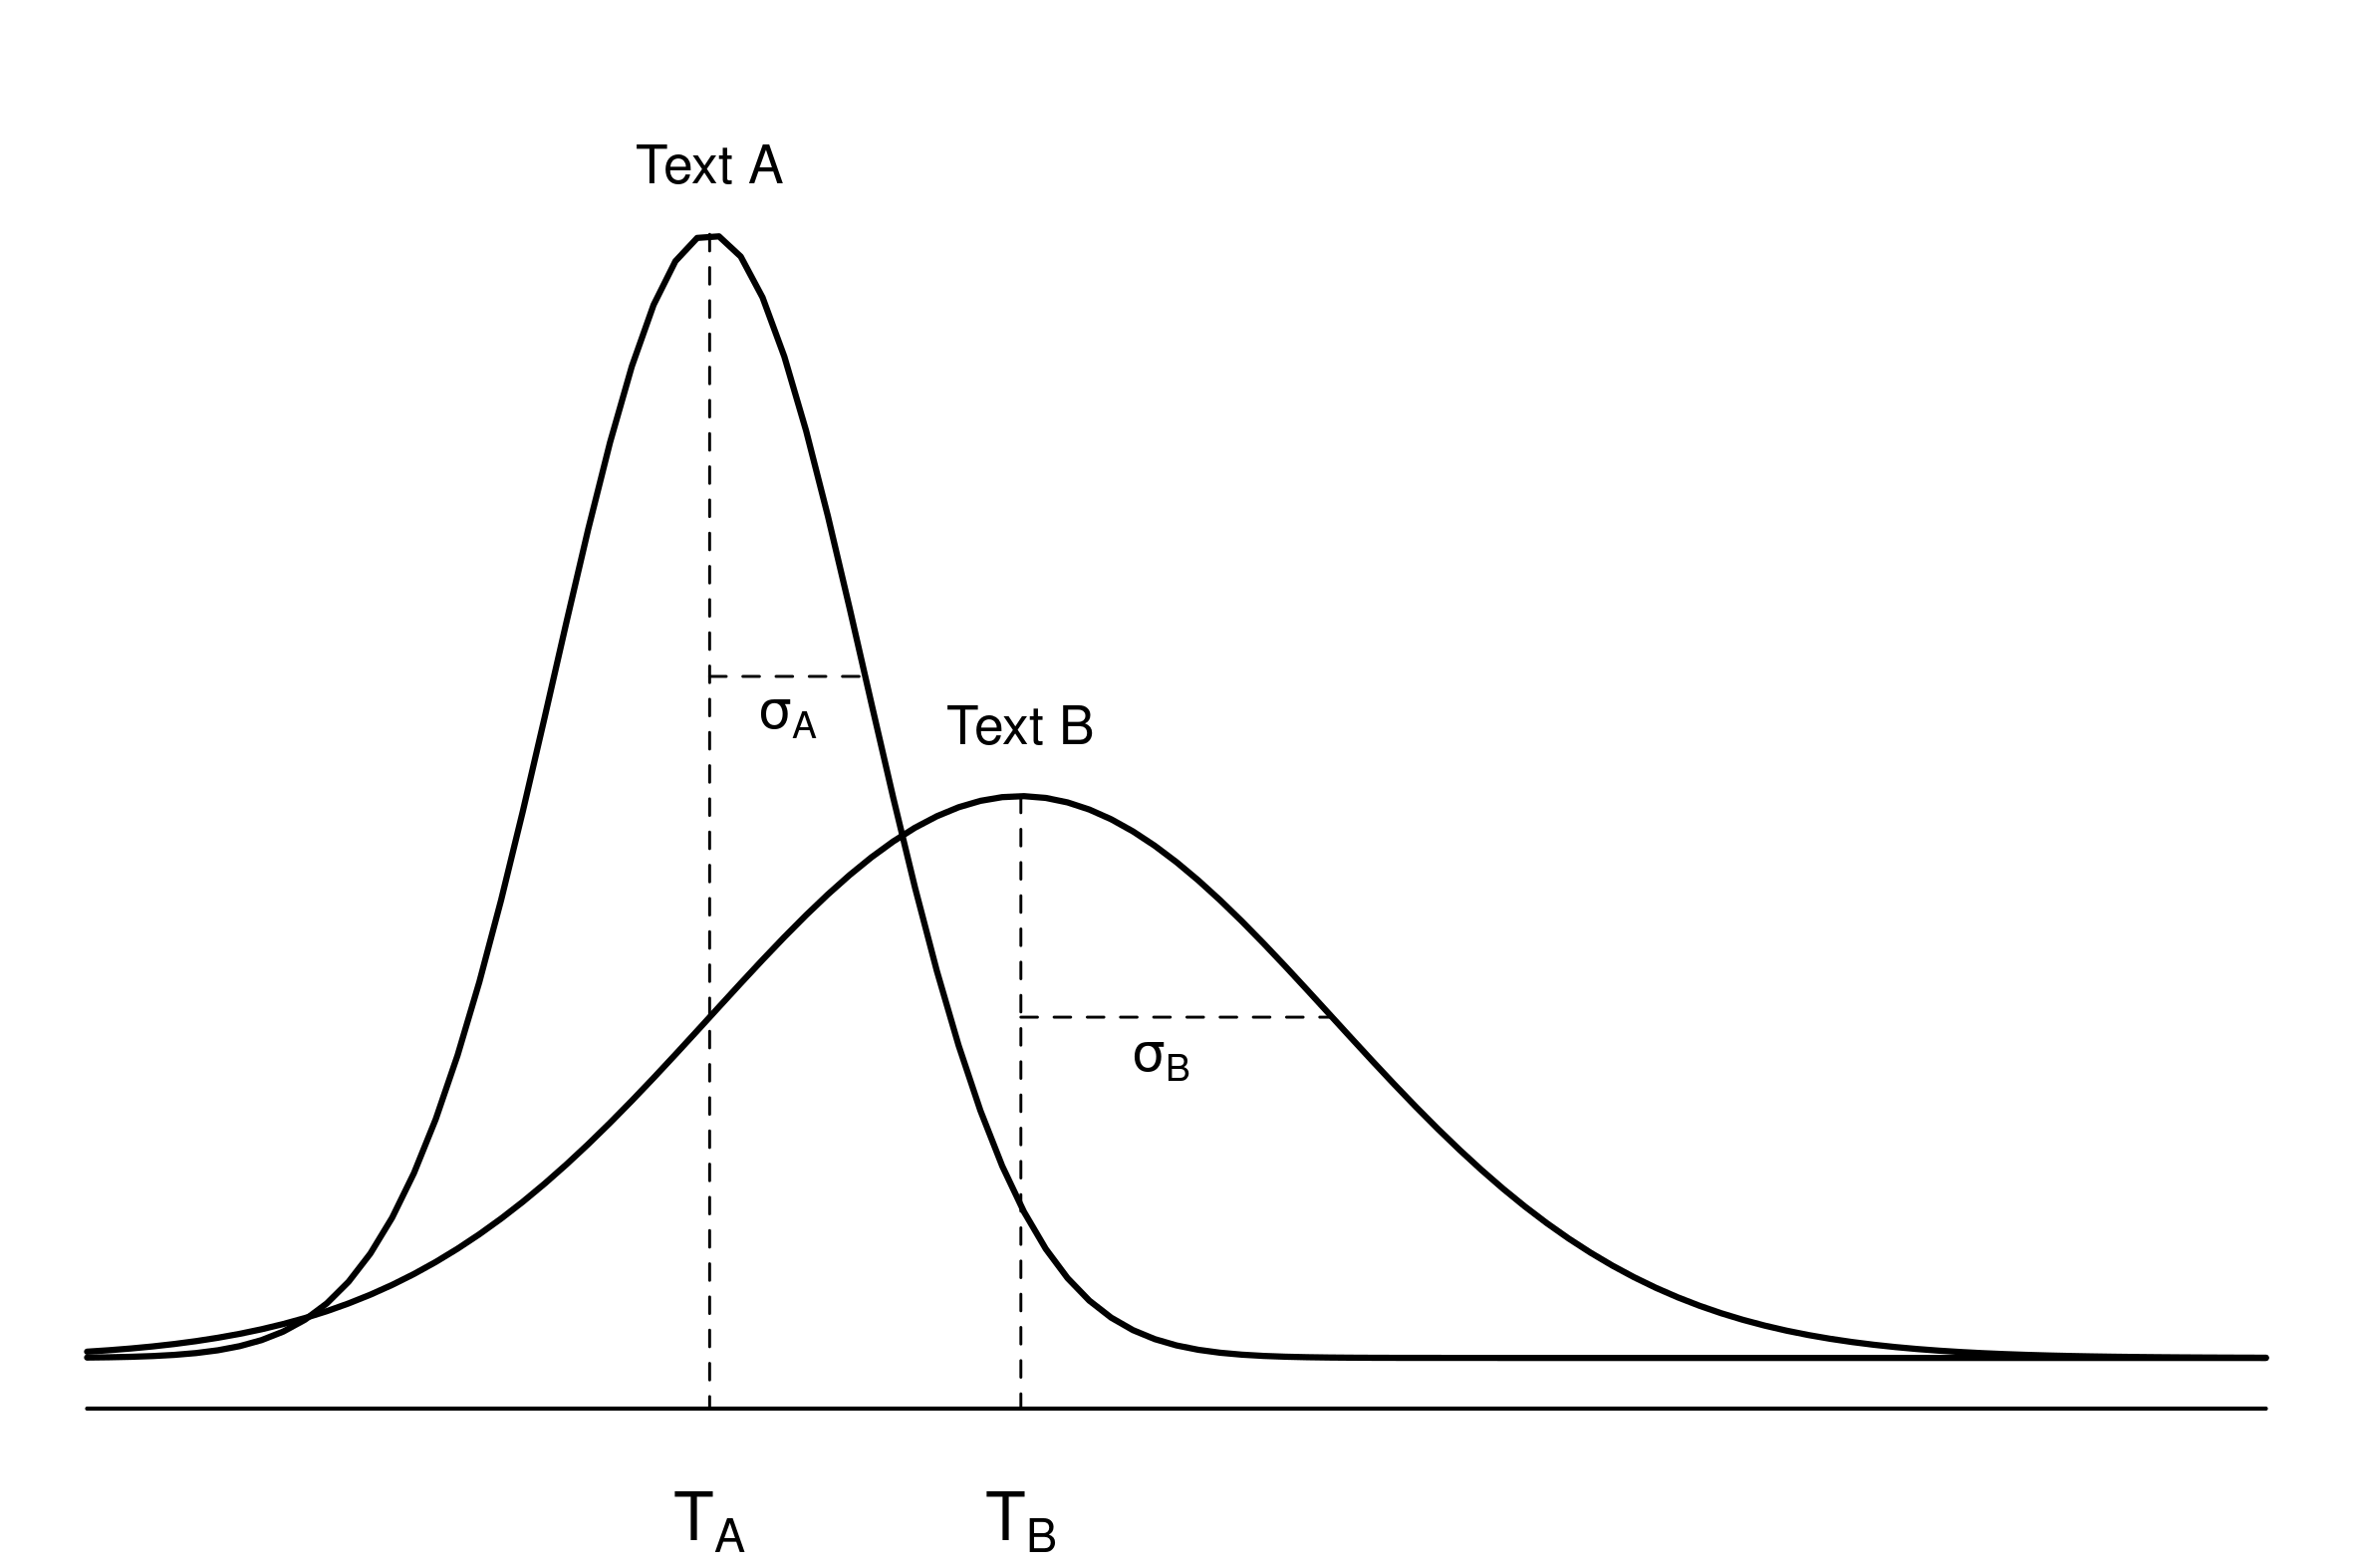
\includegraphics[width=1\linewidth,height=\textheight,keepaspectratio]{./images/png/discriminal_process.png}

}

\subcaption{\label{fig-discriminal_process}Discriminal processes}

\end{minipage}%
%
\begin{minipage}{0.50\linewidth}

\centering{

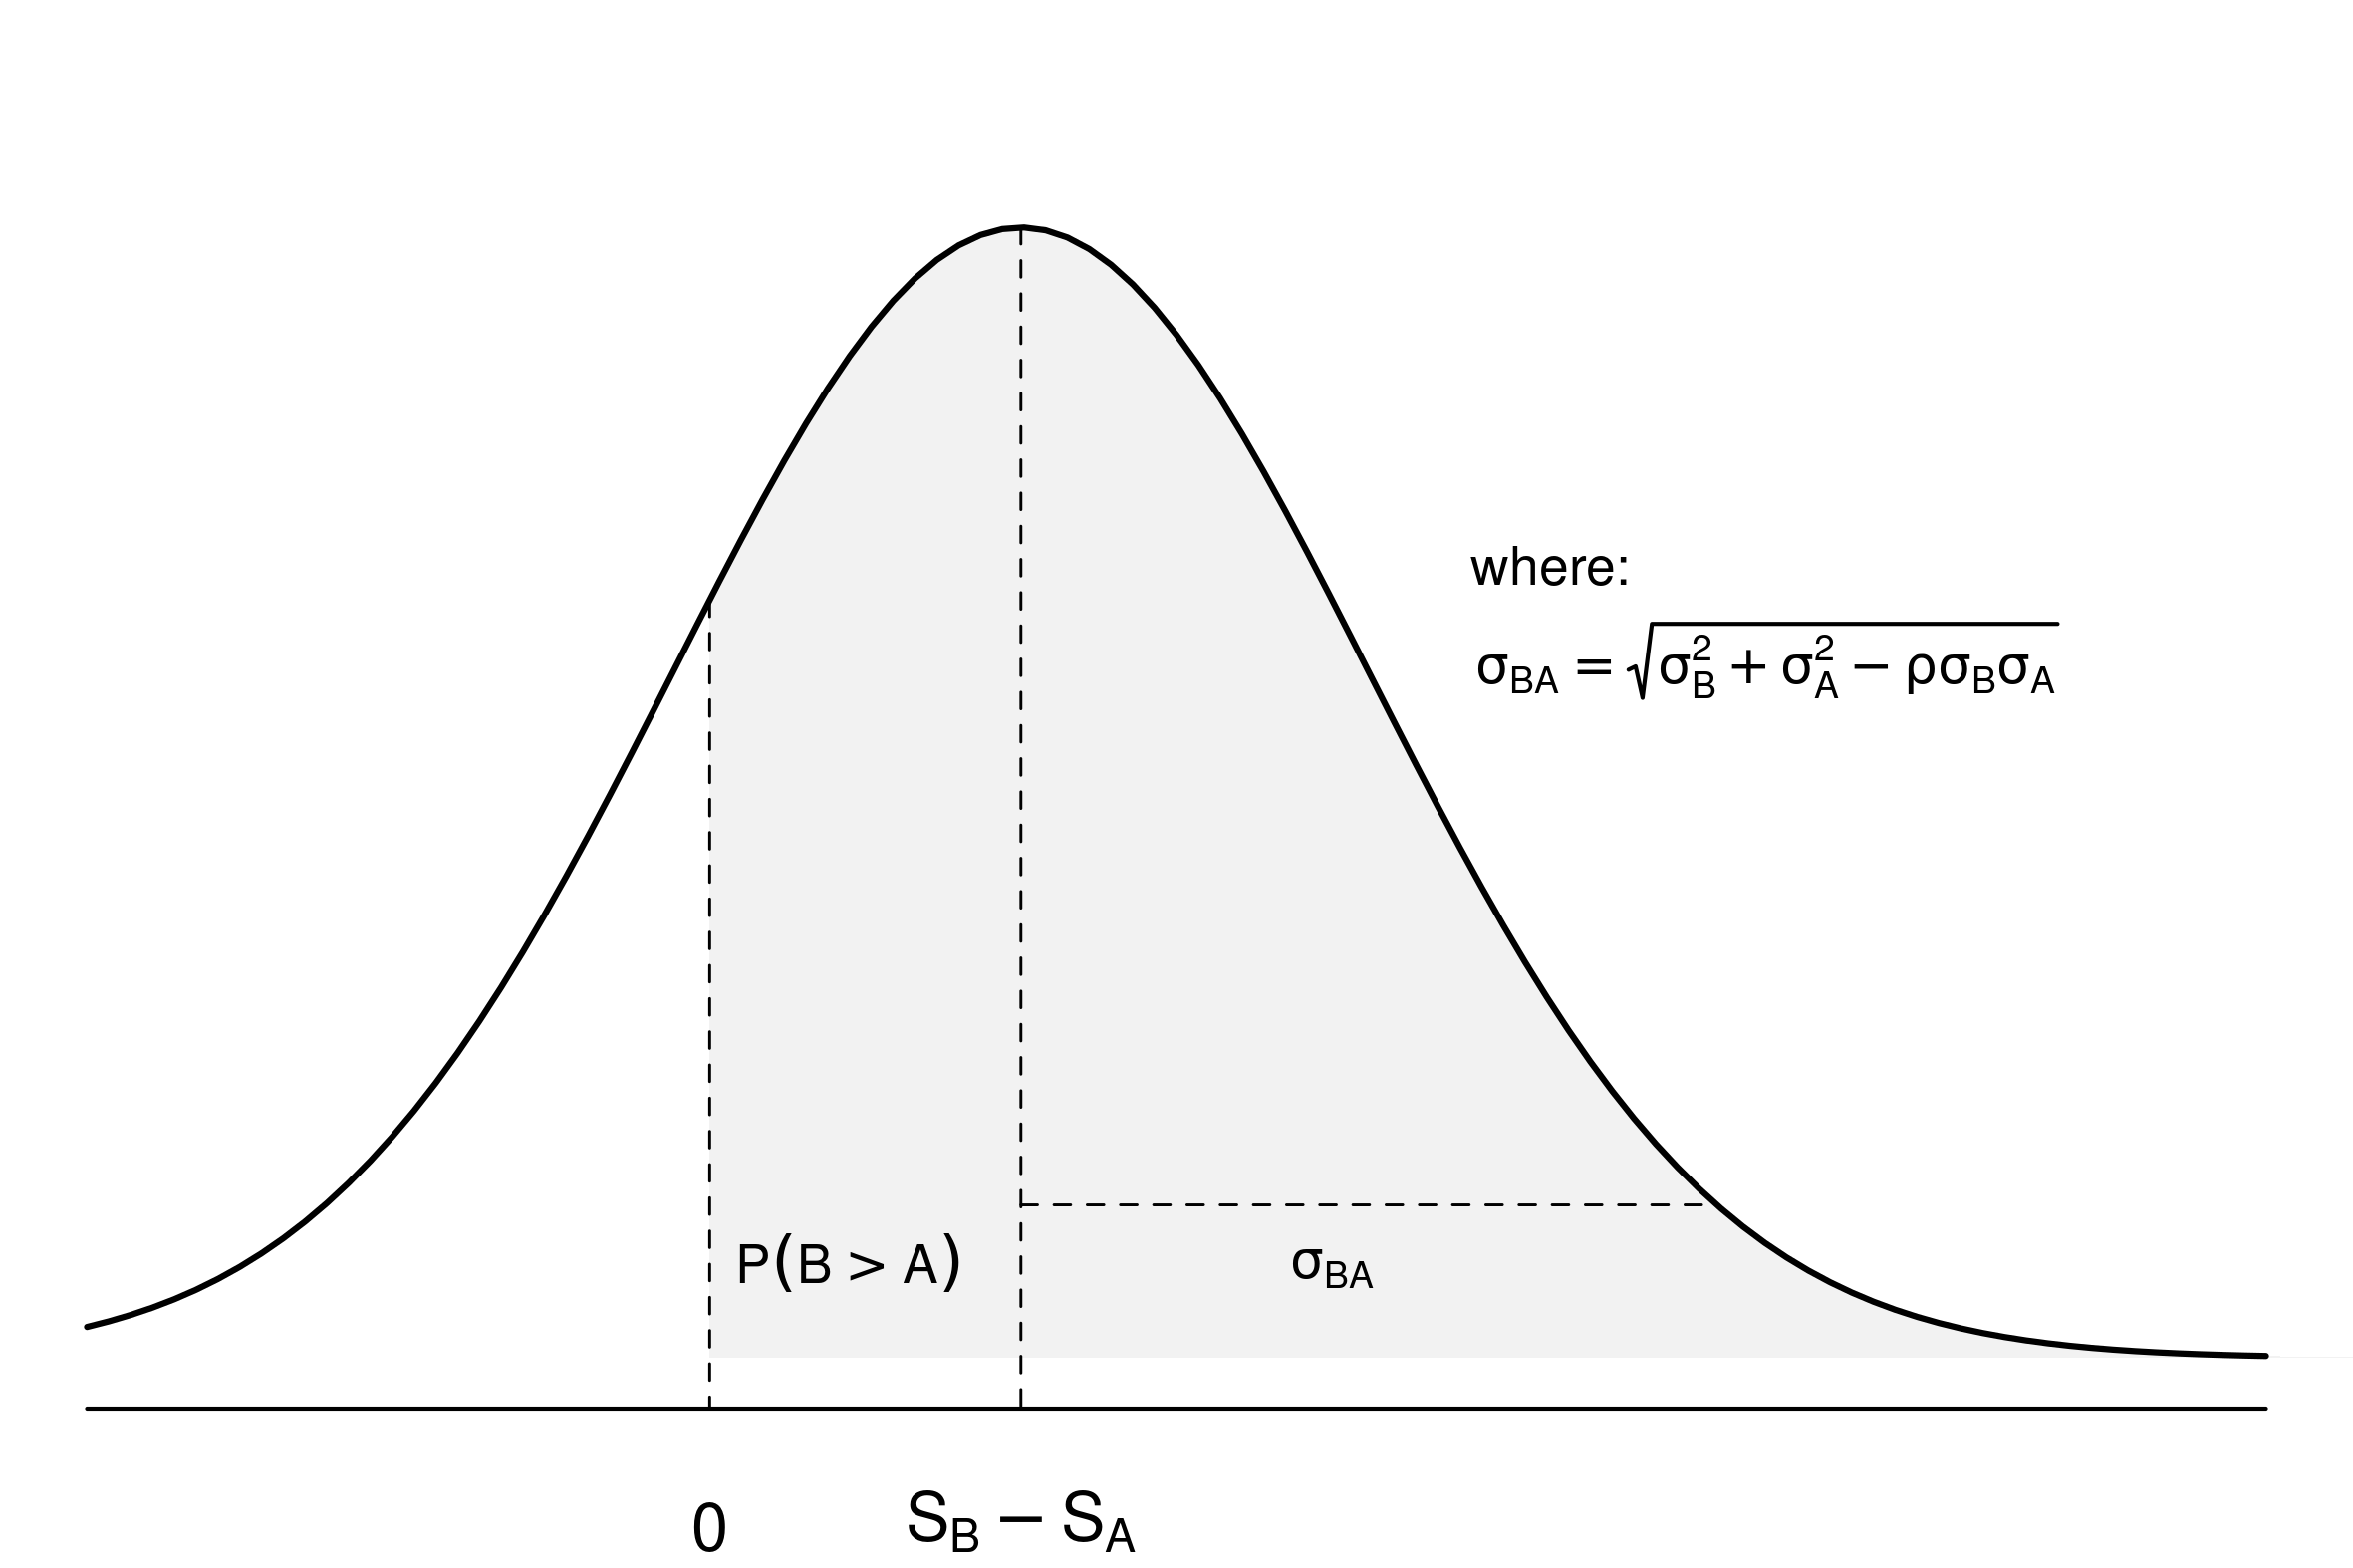
\includegraphics[width=1\linewidth,height=\textheight,keepaspectratio]{./images/png/discriminal_difference.png}

}

\subcaption{\label{fig-discriminal_difference}Discriminal difference}

\end{minipage}%

\caption{\label{fig-thurstone_theory}Hypothetical discriminal processes
and discriminant difference along a quality trait continuum for two
written texts.}

\end{figure}%

However, since the individual discriminal processes of the stimuli are
not directly observable, the theory introduces \emph{the law of
comparative judgment}. This law posits that in pairwise comparisons, a
judge perceives the stimulus with a discriminal process positioned
further along the trait continuum as possessing more of the trait
\citep[pp.~251]{Bramley_2008}. This suggests that the relative distance
between stimuli, rather than their absolute positions on the continuum,
likely defines the outcome of pairwise comparisons. Indeed, the theory
assumes that the difference between the underlying discriminal processes
of the stimuli, referred to as \emph{the discriminal difference},
determines the observed dichotomous outcome. Moreover, the theory
assumes that because the individual discriminal processes form a Normal
distribution on the continuum, the discriminal difference will also
conform to a Normal distribution \citep{Andrich_1978}. In this
distribution, the mode (mean) represents the relative separation between
the stimuli, and its dispersion indicates the variability of that
separation.

Figure~\ref{fig-discriminal_difference} illustrates the distribution of
the discriminal difference for the hypothetical texts depicted in
Figure~\ref{fig-discriminal_process}. The figure indicates that the
judge perceives Text B as having significantly higher quality than Text
A. This conclusion rests on two key observations: the positive
difference between their modal discriminal processes
\((T_{B} - T_{A} > 0)\) and the probability area where the discriminal
difference distinctly favors Text B over Text A, represented by the
shaded gray area denoted as \(P(B > A)\). As a result, the dichotomous
outcome of this comparison is more likely to favor Text B over Text A.

\section{The two critical issues in CJ
literature}\label{sec-theory-issues}

This section examines the two critical issues in the CJ literature that
serve as the primary focus of this study. The first is the overreliance
on Thurstone's Case V assumptions in the statistical analysis of CJ
data. The second is the apparent disconnect between CJ's approach to
trait measurement and hypothesis testing.

\subsection{The Case V and the statistical analysis of CJ
data}\label{sec-theory-issue1}

Thurstone noted that the general form of the theory, as delineated in
Section~\ref{sec-thurstone_theory}, gave rise to a trait scaling
problem. The model required estimating more ``unknown'' parameters than
the available pairwise comparisons \citep[pp.~267]{Thurstone_1927b}. To
address this issue and facilitate the practical implementation of the
theory, he developed five cases derived from this general form, each
case progressively incorporated additional simplifying assumptions into
the model.

In Case I, Thurstone postulated that pairs of stimuli would maintain a
constant correlation across all comparisons. In Case II, he allowed
multiple judges to undertake comparisons instead of confining
evaluations to a single judge. In Case III, he posited that there was no
correlation between stimuli. In Case IV, he assumed that the stimuli
exhibited similar dispersions. Finally, in Case V, he replaced this
assumption with the condition that stimuli had equal discriminal
dispersions. Table~\ref{tbl-thurstone_cases} summarizes the assumptions
of the general form and the five cases. For a detailed discussion of
these cases and their progression, refer to \citet{Thurstone_1927b} and
\citet[pp.~248--253]{Bramley_2008}.

\begin{table}

\caption{\label{tbl-thurstone_cases}Thurstones cases and their
asumptions}

\centering{

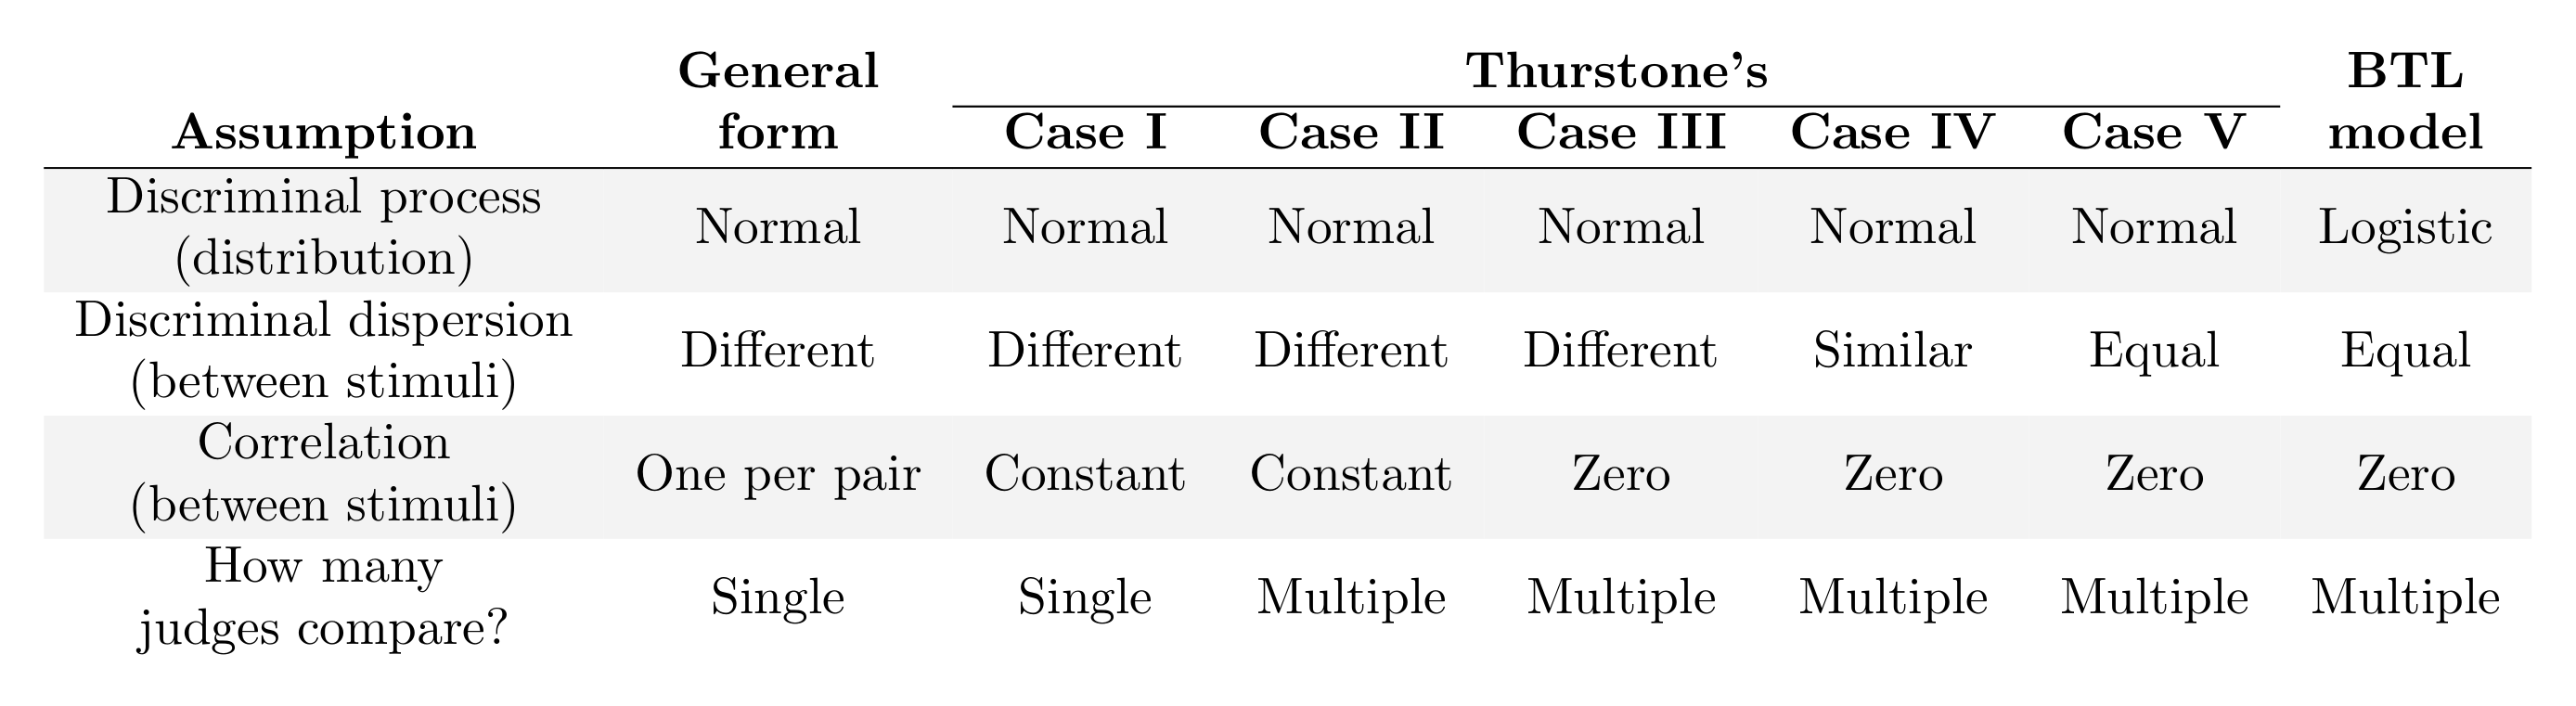
\includegraphics[width=1\linewidth,height=\textheight,keepaspectratio]{./images/png/thurstone_cases.png}

}

\end{table}%

Despite relying on the most extensive set of simplifying assumptions
\citetext{\citealp[pp.~253]{Bramley_2008}; \citealp[pp.~677]{Kelly_et_al_2022}},
Case V remains the most widely used case in the CJ literature. This
popularity stems mainly from its simplified statistical representation
in the Bradley-Terry-Luce (BTL) model
\citep{Bradley_et_al_1952, Luce_1959}. The BTL model mirrors the
assumptions of Case V, with one notable distinction: whereas Case V
assumes a Normal distribution for the stimuli's discriminal processes,
the BTL model uses the more mathematically tractable Logistic
distribution \citep[pp.~254]{Andrich_1978, Bramley_2008} (see
Table~\ref{tbl-thurstone_cases}). This substitution has little impact on
the model's estimation or interpretation, as the Normal and Logistic
distributions exhibit analogous statistical properties, differing only
by a scaling factor of approximately \(1.7\)
\citep[pp.~16]{vanderLinden_et_al_2017_I}.

However, Thurstone originally developed Case V to provide a ``rather
coarse scaling'' of traits \citep[pp.~269]{Thurstone_1927b},
prioritizing statistical simplicity over precision in trait measurement
\citep[pp.~677]{Kelly_et_al_2022}. He explicitly warned against its
untested application, stating that its use ``should not be made without
(an) experimental test'' \citep[pp.~270]{Thurstone_1927b}. Furthermore,
he acknowledged that some assumptions could prove problematic when
researchers assess complex traits or heterogeneous stimuli
\citep[pp.~376]{Thurstone_1927a}. Consequently, given that modern CJ
applications frequently involve such traits and stimuli, two main
assumptions of Case V and, by extension, of the BTL model may not
consistently hold in theory or practice, namely the assumption of equal
dispersion and zero correlation between stimuli.

\subsubsection{The assumption of equal dispersions between
stimuli}\label{sec-theory-issue1a}

According to the theory, discrepancies in the discriminal dispersions of
stimuli shape the distribution of the discriminal difference, exerting a
direct influence on the outcome of pairwise comparisons.
Figure~\ref{fig-dispersion} presents a thought experiment to illustrate
this idea. In this experiment, a researcher can observe the discriminal
processes for the texts depicted in
Figure~\ref{fig-discriminal_process}. Furthermore, the figure assumes
that the discriminal dispersion for Text A remains constant and that the
texts are uncorrelated \((\rho=0)\). The figure reveals that an increase
in the uncertainty associated with the perception of Text B in
comparison to Text A, \((\sigma_{B}-\sigma_{A})\), broadens the
distribution of their discriminal difference. This broadening affects
the probability area where the discriminal difference distinctly favors
Text B over Text A, expressed as \(P(B > A)\), ultimately influencing
the comparison outcome. Additionally, the figure reveals that when the
discriminal dispersions of the texts are equal
\((\sigma_{B}-\sigma_{A}=0)\), the discriminal difference is more likely
to favor Text B over Text A (shaded gray area), compared to situations
where their dispersions differ.

In experimental practice, however, this process occurs in reverse.
Researchers first observe the comparison outcome and then use the BTL
model to infer the discriminal difference between the stimuli and their
respective discriminal processes \citep[pp.~373]{Thurstone_1927a}.
Therefore, it is reasonable to assume that the outcome's ability to
reflect the ``true'' differences between stimuli largely depends on the
validity of the model's assumptions, particularly the assumption of
equal dispersions. For instance, when researchers observe a sample of
outcomes favoring Text B over Text A and correctly assume equal
dispersions between the texts, the BTL model estimates a discriminal
difference distribution that accurately represents the ``true''
discriminal difference of the texts. This scenario is illustrated in
Figure~\ref{fig-dispersion}, where the model's discriminal difference
distribution aligns with the ``true'' distribution, represented by the
thick continuous line corresponding to \(\sigma_{B}-\sigma_{A}=0\). The
accuracy of these discriminal difference ensures reliable estimates for
the texts' discriminal processes {(citation needed?)}.

However, Thurstone argued that the assumption of equal dispersions may
not be applicable when researchers assess complex traits or
heterogeneous stimuli \citep[pp.~376]{Thurstone_1927a}, as these traits
and stimuli can introduce judgment discrepancies due to their unique
features
\citep{vanDaal_et_al_2016, Lesterhuis_2018, Chambers_et_al_2022}.
Indeed, evidence of this violation may already be present in the CJ
literature in the form of misfit statistics, which measure judgment
discrepancies associated with specific stimuli
\citetext{\citealp[pp.~12]{Pollitt_2004}; \citealp[pp.~20]{Goossens_et_al_2018}}.
For example, labeling texts as ``misfits'' indicates that comparisons
involving these texts result in more judgment discrepancies than those
involving other texts
\citep{Pollitt_2012a, Pollitt_2012b, vanDaal_et_al_2016, Goossens_et_al_2018}.
These discrepancies, in turn, suggest that the discriminal differences
for ``misfit'' texts have broader distributions, indicating that their
discriminal processes may also exhibit more variation than that of other
texts. A similar line of reasoning applies to the concept of ``misfit''
judges, whose evaluations deviate substantially from the shared
consensus due to the unique characteristics of the stimuli or the judges
themselves. These ``misfit'' judges and their associated deviations can
give rise to additional statistical and measurement issues, which we
discuss in more detail in Section~\ref{sec-theory-issue1b}.

Nevertheless, model misspecification, in the form of an erroneous
assumption of equal dispersions between stimuli, can give rise to
significant statistical and measurement issues. For instance, the model
may overestimate the degree to which the outcome accurately reflects the
``true'' discriminal differences between stimuli. This overestimation
can result in researchers drawing spurious conclusions about these
differences \citep[pp.~370]{McElreath_2020} and, by extension, about the
underlying discriminal processes of stimuli. Figure~\ref{fig-dispersion}
illustrates this issue when the model's discriminal difference
distribution aligns with the thick continuous line for
\(\sigma_{B}-\sigma_{A}=0\), while the ``true'' discriminal difference
follows any discontinuous line where \(\sigma_{B}-\sigma_{A} \neq 0\).

Additionally, if researchers recognize that misfit statistics highlight
these critical differences in dispersions, the conventional CJ practice
of excluding stimuli based on these statistics
\citep{Pollitt_2012a, Pollitt_2012b, vanDaal_et_al_2016, Goossens_et_al_2018}
can unintentionally discard valuable information. Such exclusions can
introduce bias into trait estimates
\citep[chap.~12]{Zimmerman_1994, McElreath_2020}. The direction and
magnitude of these biases are often unpredictable, as they depend on
which stimuli are excluded from the analysis.

\begin{figure}

\begin{minipage}{0.50\linewidth}

\centering{

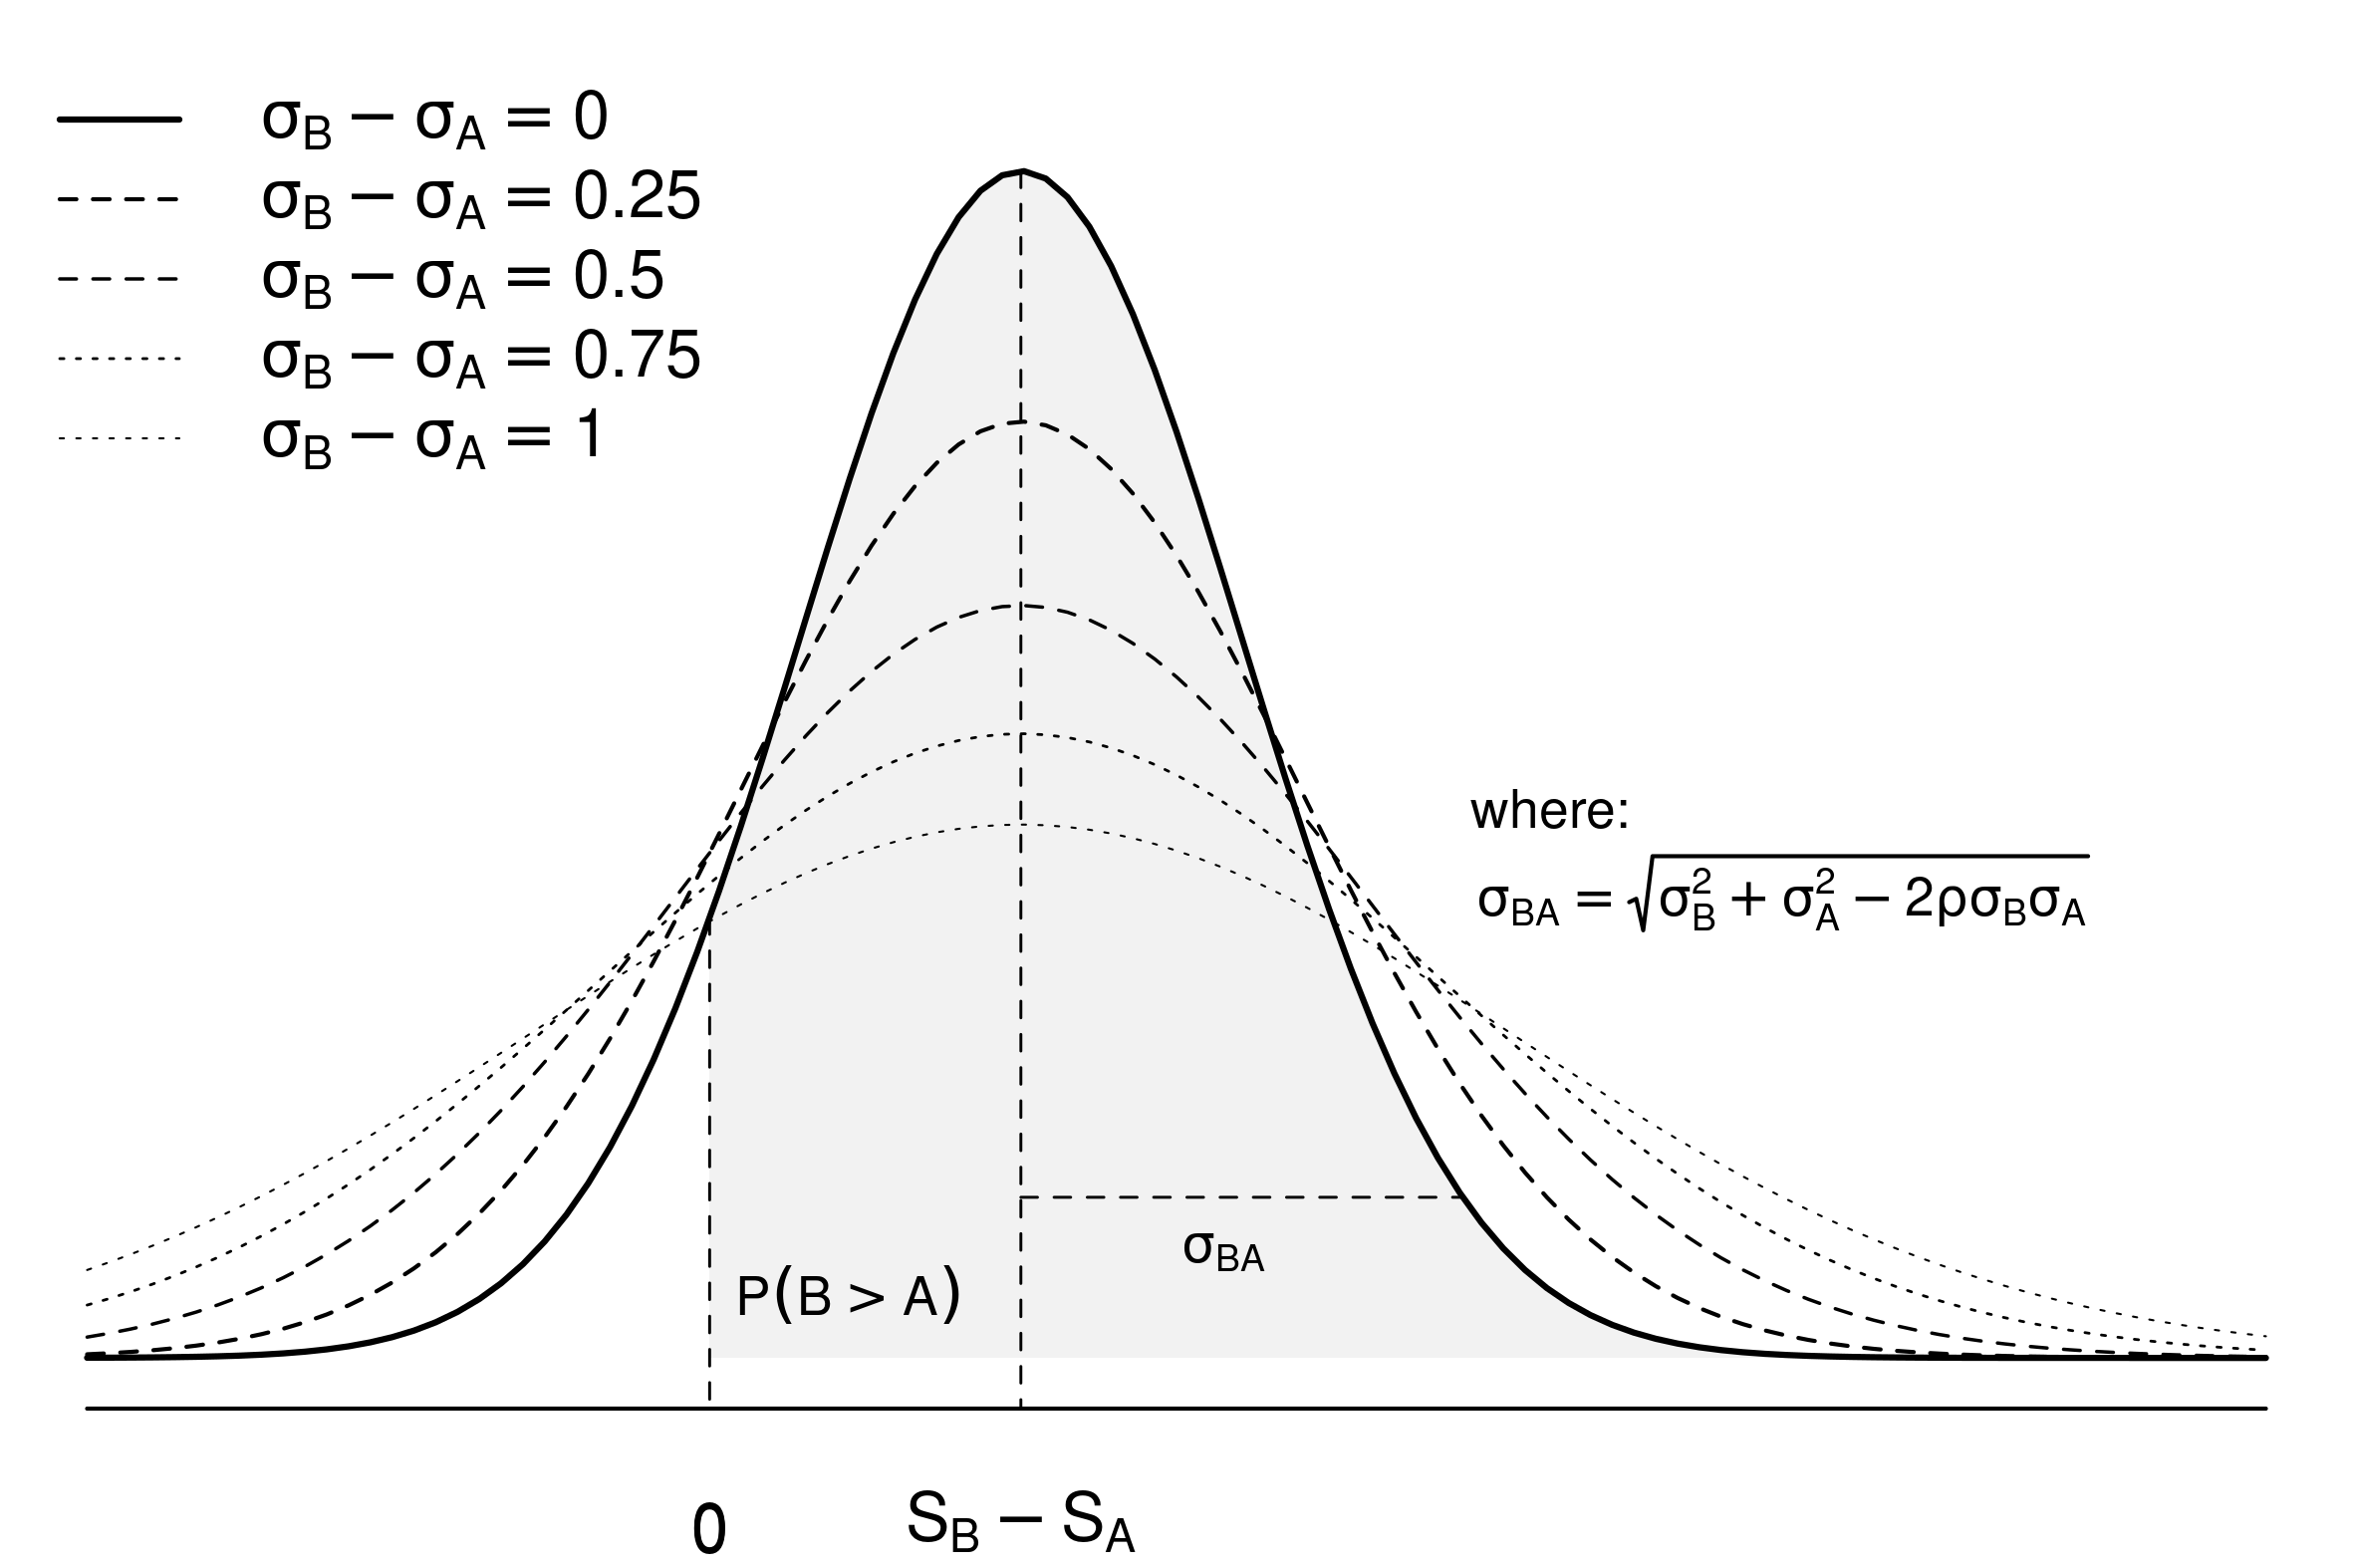
\includegraphics[width=1\linewidth,height=\textheight,keepaspectratio]{./images/png/dispersion.png}

}

\subcaption{\label{fig-dispersion}Discrepancies in the dispersions of
stimuli}

\end{minipage}%
%
\begin{minipage}{0.50\linewidth}

\centering{

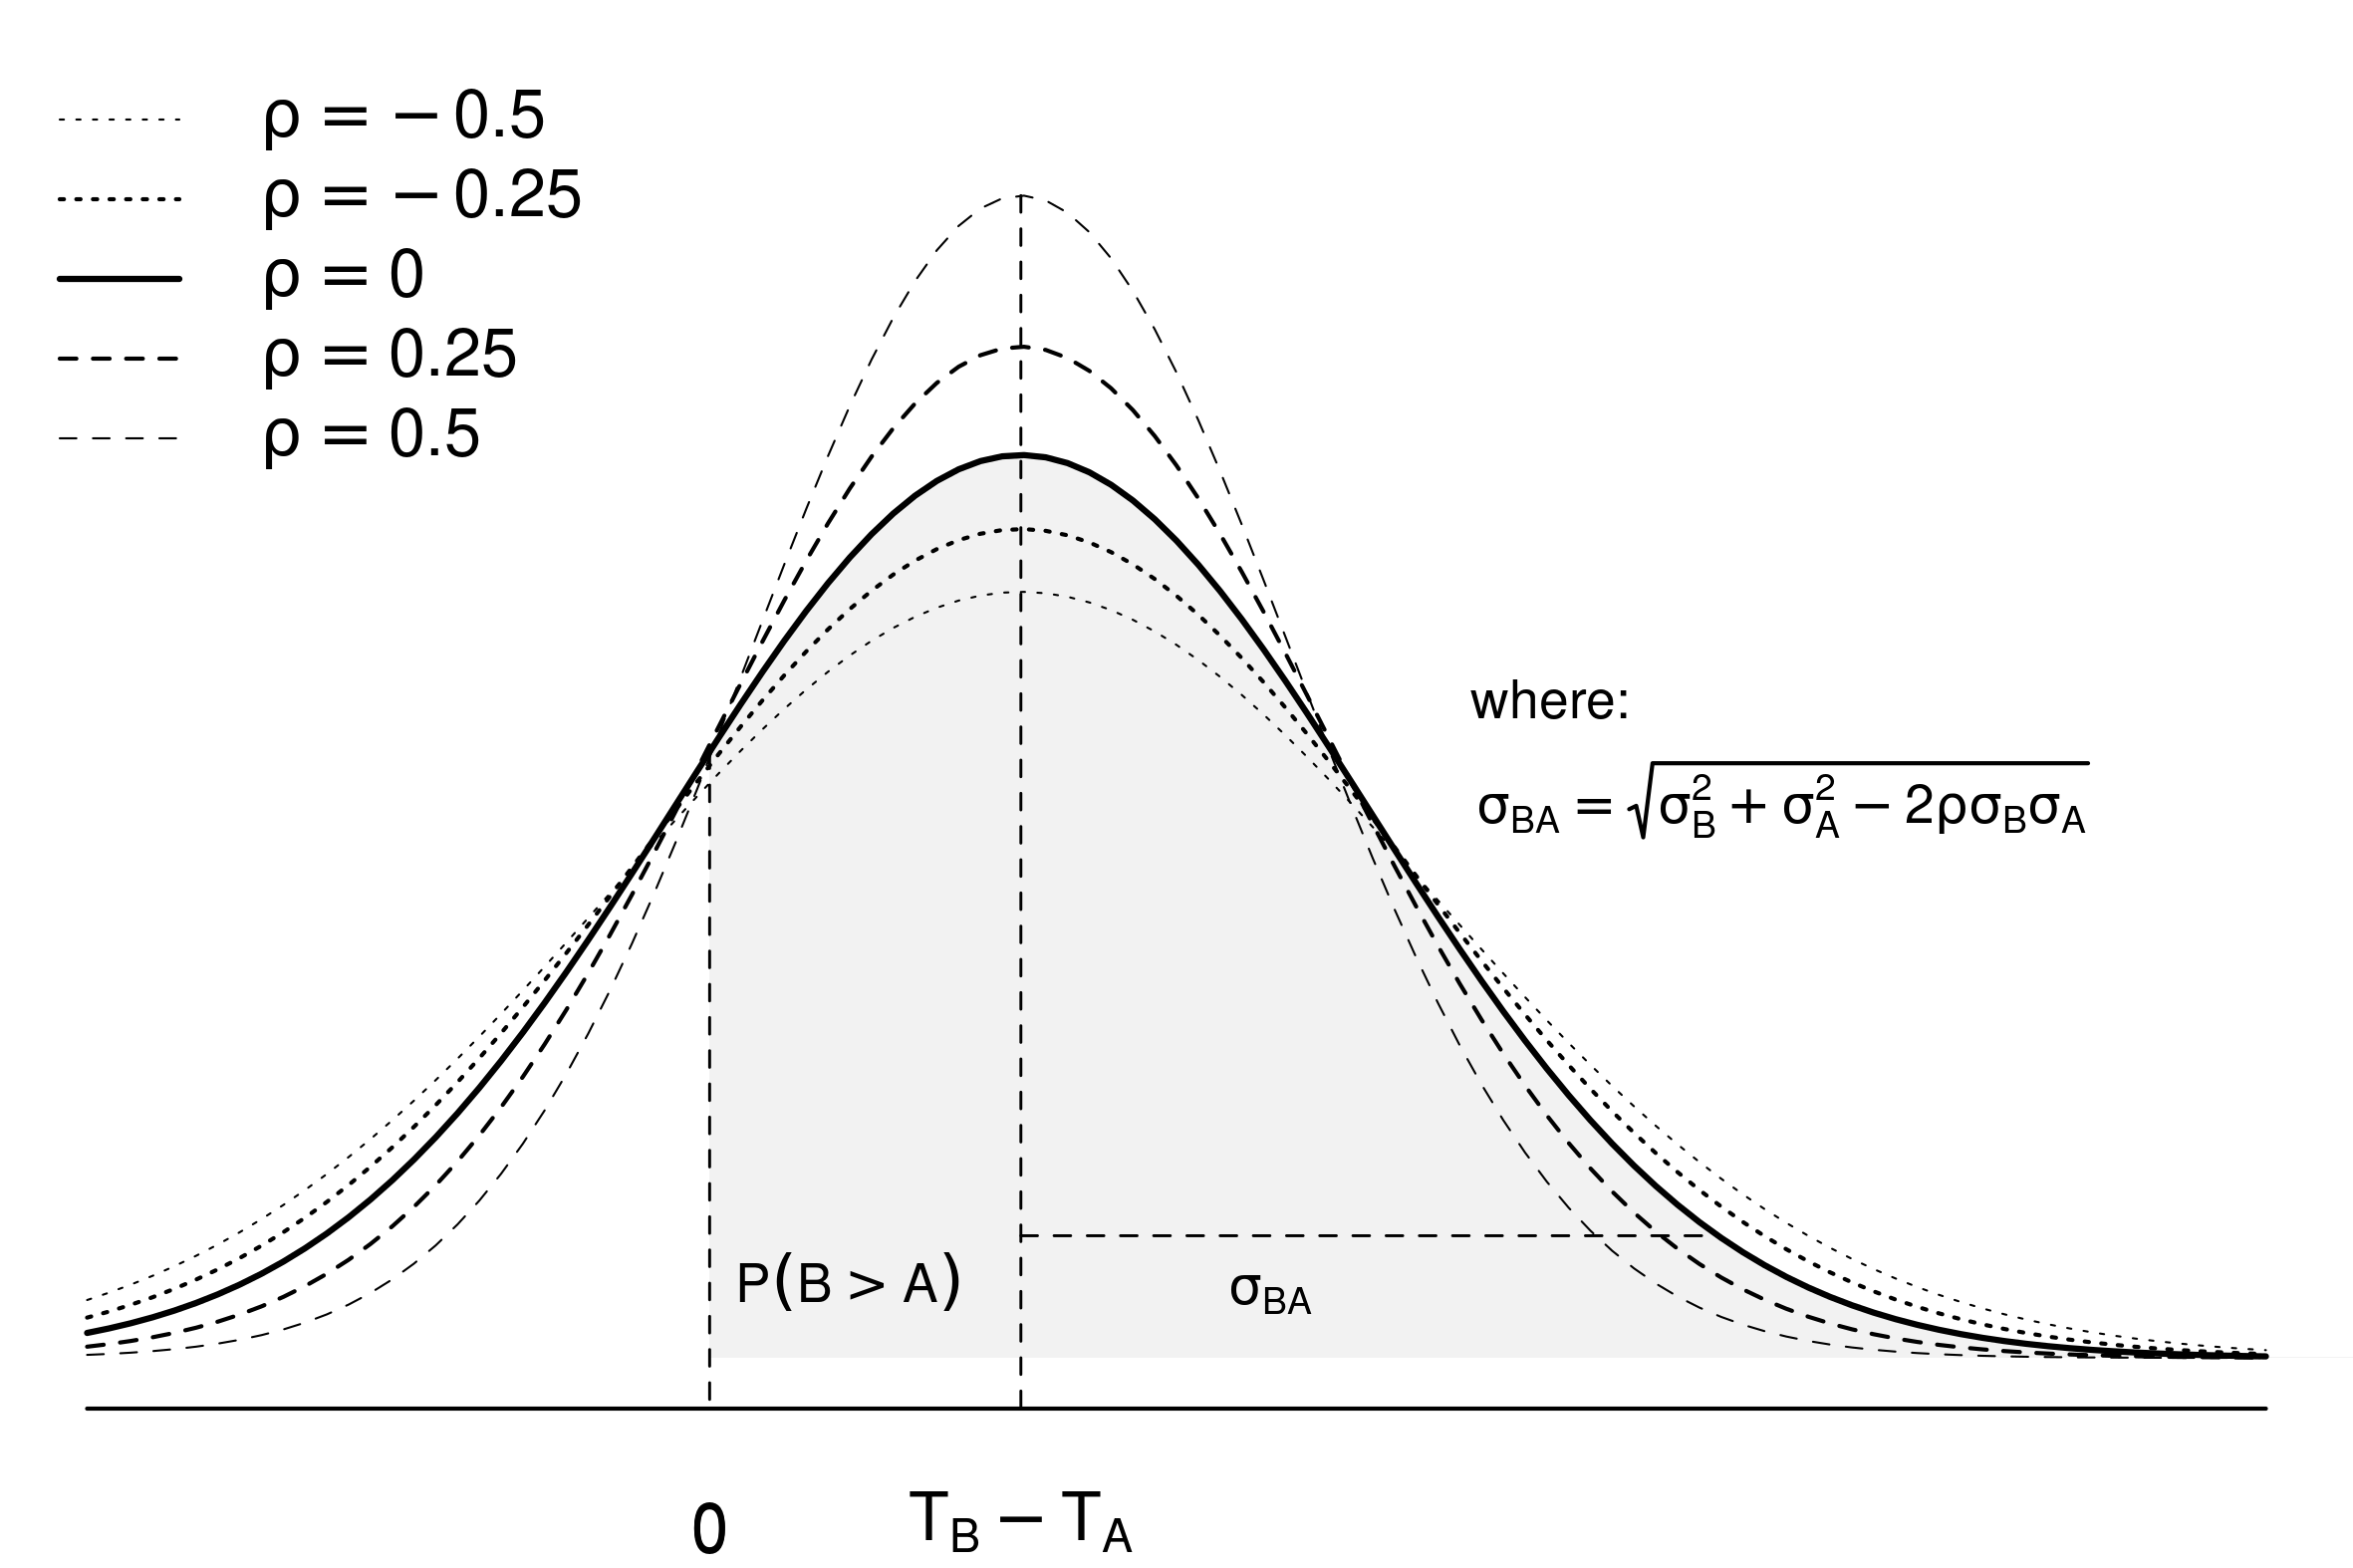
\includegraphics[width=1\linewidth,height=\textheight,keepaspectratio]{./images/png/correlation.png}

}

\subcaption{\label{fig-correlation}Correlation between stimuli}

\end{minipage}%

\caption{\label{fig-caseV_issues}The effect of dispersion discrepancies
and stimulus correlation on the distribution of the discriminal
difference.}

\end{figure}%

\subsubsection{The assumption of zero correlation between
stimuli}\label{sec-theory-issue1b}

The correlation, represented by the symbol \(\rho\), measures how much a
judge's perception of a specific trait in one stimulus depends on their
perception of the same trait in another. As with the discriminal
dispersions, this correlation shapes the distribution of the discriminal
difference, directly impacting the outcomes of pairwise comparisons.
Figure~\ref{fig-correlation} presents a similar thought experiment as in
Section~\ref{sec-theory-issue1a} to illustrate this idea. The
illustration now assumes that the discriminal dispersions for both texts
remain constant. The figure shows that as the correlation between the
texts increases, the distribution of their discriminal difference
becomes narrower. This narrowing affects the area under the curve where
the discriminal difference distinctly favors Text B over Text A, denoted
as \(P(B > A)\), thus influencing the comparison outcome. Furthermore,
the figure shows that when two texts are independent or uncorrelated
\((\rho=0)\), their discriminal difference is less likely to favor Text
B over Text A (shaded gray area) compared to scenarios where the texts
are highly correlated.

However, in practice, researchers approach this process in reverse. They
begin by observing the sample of outcomes favoring Text B over Text A
and then use the BTL model to estimate the discriminal difference and
the discriminal processes of the stimuli. Given that the BTL model
assumes independent discriminal processes across comparisons, if this
assumption holds, then the model estimates a discriminal difference
distribution that accurately reflects the ``true'' discriminal
difference of the texts. This scenario is illustrated with
Figure~\ref{fig-correlation} when the discriminal difference
distribution of the model aligns with the ``true'' distribution,
represented by the thick continuous line corresponding to \(\rho=0\).
Once more, the estimation accuracy of the discriminal difference ensures
reliable estimates for the discriminal processes of the texts {(citation
needed?)}.

Notably, Thurstone attributed the independence of stimuli to the
cancellation of potential judges' biases. He argued that this
cancellation resulted from two opposing and equally weighted effects
occurring during pairwise comparisons \citep[pp.~268]{Thurstone_1927b}.
\citet{Andrich_1978} provided a mathematical demonstration of this
cancellation using the BTL model under the assumption of discriminal
processes with additive biases. However, it is easy to imagine at least
two scenarios in which the zero correlation assumption is almost
certainly invalid: when the pairwise comparison involves
multidimensional, complex traits with heterogeneous stimuli and when an
additional hierarchical structure is relevant to the stimuli.

In the first scenario, the intricate aspects of multidimensional,
complex traits may introduce dependencies between the stimuli due to
certain judges' biases that resist cancellation. Research on text
quality suggests that when judges evaluate these traits, they often rely
on various intricate characteristics of the stimuli to form their
judgments
\citep{vanDaal_et_al_2016, Lesterhuis_2018, Chambers_et_al_2022}. These
additional relevant characteristics, which are unlikely to be equally
weighted or opposing, can exert an uneven influence on judges'
perceptions, creating biases in their judgments and, ultimately,
introducing dependencies between stimuli
\citep[pp.~346]{vanderLinden_et_al_2017_II}. For example, this could
occur when a judge assessing the argumentative quality of a text places
more weight on its grammatical accuracy than other judges, thereby
favoring texts with fewer errors but weaker arguments. While direct
evidence for this particular scenario is lacking, studies such as
\citet{Pollitt_et_al_2003} demonstrate the presence of such biases,
supporting the notion that the factors influencing pairwise comparisons
may not always cancel out.

In the second scenario, the shared context or inherent connections
created by additional hierarchical structures may further introduce
dependencies between stimuli, a statistical phenomenon commonly known as
clustering \citep{Everitt_et_al_2010}. Despite the CJ literature
acknowledging the existence of such hierarchical structures, the
statistical handling of this additional source of dependence between
stimuli has been inadequate. For instance, when CJ data incorporates
multiple samples of stimuli from the same individuals, researchers
frequently rely on (average) estimated BTL scores to conduct subsequent
analyses and tests at the individual hierarchical level
\citep{Bramley_et_al_2019, Boonen_et_al_2020, Bouwer_et_al_2023, vanDaal_et_al_2017, Jones_et_al_2019, Gijsen_et_al_2021}.
However, this approach can introduce additional statistical and
measurement issues, which we discuss in greater detail in
Section~\ref{sec-theory-issue2}.

In any case, similar to Section~\ref{sec-theory-issue1a}, model
misspecification due to an erroneous assumption of zero correlation
between stimuli can lead to significant statistical and measurement
issues. For instance, the model may over- or underestimate how
accurately the outcome reflects the ``true'' discriminal differences
between stimuli. Such inaccuracies can result in spurious inferences
about these differences and, by extension, about the stimuli's
discriminal processes. This scenario is illustrated in
Figure~\ref{fig-correlation}, where the model's discriminal difference
distribution aligns with the thick continuous line for \(\rho=0\), while
the ``true'' discriminal difference follows any discontinuous line where
\(\rho \neq 0\).

This misspecification may arise from neglecting additional relevant
traits, excluding judges based on misfit statistics, or ignoring
hierarchical (grouping) structures. Neglecting relevant traits, such as
judges' biases, can cause dimensional mismatches in the BTL model,
artificially inflating the trait's reliability
\citep[pp.~341]{Hoyle_et_al_2023} or, worse, introducing bias into the
trait's estimates \citep{Ackerman_1989}. Excluding judges based on
misfit statistics risks discarding valuable information, which may
further bias the trait's estimates
\citep[chap.~12]{Zimmerman_1994, McElreath_2020}. Finally, ignoring
hierarchical structures may reduce the precision of model parameter
estimates, potentially amplifying the overestimation of the trait's
reliability \citep[pp.~482]{Hoyle_et_al_2023}.

\subsection{The disconnect between trait measurement and hypothesis
testing}\label{sec-theory-issue2}

Building on the previous section, it is clear that, despite its
limitations, the BTL model is commonly used as the measurement model in
CJ assessments. A measurement model specifies how manifest variables
contribute to the estimation of latent variables
\citep{Everitt_et_al_2010}. For example, when evaluating text quality,
researchers use the BTL model to process the dichotomous outcomes
resulting from the pairwise comparisons (the manifest variables) to
estimate scores that reflect the underlying quality level of the texts
(the latent variable)
\citep{Laming_2004, Pollitt_2012b, Whitehouse_2012, vanDaal_et_al_2016, Lesterhuis_2018_thesis, Coertjens_et_al_2017, Goossens_et_al_2018, Bouwer_et_al_2023}.

Researchers then typically use these estimated BTL scores, or their
transformations, to conduct additional analyses or hypothesis tests. For
example, these scores have been used to identify `misfit' judges and
stimuli \citep{Pollitt_2012b, vanDaal_et_al_2016, Goossens_et_al_2018},
detect biases in judges' ratings
\citep{Pollitt_et_al_2003, Pollitt_2012b}, calculate correlations with
other assessment methods \citep{Goossens_et_al_2018, Bouwer_et_al_2023},
or test hypotheses related to the underlying trait of interest
\citep{Bramley_et_al_2019, Boonen_et_al_2020, Bouwer_et_al_2023, vanDaal_et_al_2017, Jones_et_al_2019, Gijsen_et_al_2021}.

However, the statistical literature advises caution when using estimated
scores for additional analyses and tests. A key consideration is that
BTL scores are parameter estimates that inherently carry uncertainty.
Ignoring this uncertainty can bias the analysis and reduce the precision
of hypothesis tests. Notably, the direction and magnitude of such biases
are often unpredictable. Results may be attenuated, exaggerated, or
remain unaffected depending on the degree of uncertainty in the scores
and the actual effects being tested
\citetext{\citealp[pp.~25]{Kline_et_al_2023}; \citealp[pp.~137]{Hoyle_et_al_2023}}.
Finally, the reduced precision in hypothesis tests diminishes their
statistical power, increasing the likelihood of committing type-I or
type-II errors \citep{McElreath_2020}.

In aggregate, researchers' inadequate handling of violations to the
assumptions of equal dispersion and zero correlation between stimuli,
coupled with the apparent disconnect between CJ's approach to trait
measurement and hypothesis testing, can potentially compromise the
reliability of the trait estimates and, by extension, their validity
\citep[pp.~2]{Perron_et_al_2015}. Consequently, adopting a more
systematic and integrated approach to examine the factors influencing CJ
experiments could offer several statistical and measurement benefits,
including the ability to address these issues.

\section{An updated theoretical and statistical model for
CJ}\label{sec-theory}

This section introduces a theoretical model for Comparative Judgment
(CJ) that builds upon Thurstone's theory. The model systematically
accounts for the factors influencing judges during CJ experiments. These
theoretical and practical insights are then translated into a
statistical model.

\subsection{The theoretical model}\label{sec-theory-theoretical}

The (latent) discriminal difference of the stimuli directly determines
the (manifest) outcome of the pairwise comparisons

The (latent) ``perceived'' discriminal processes for the stimuli
directly determines their discriminal difference

The (latent) ``true'' discriminal processes for the stimuli and the
judges' biases directly determines their (latent) ``perceived''
discriminal processes

\paragraph{Figure 3}

\begin{figure}

\centering{

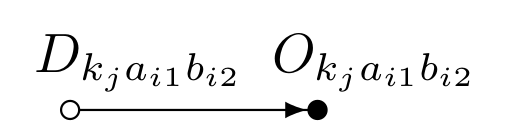
\includegraphics[width=0.2\linewidth,height=\textheight,keepaspectratio]{./images/png/CJ_TM_A1.png}

}

\caption{\label{fig-CJ_TM_A1}}

\end{figure}%

\paragraph{Figure 4}

\begin{figure}

\centering{

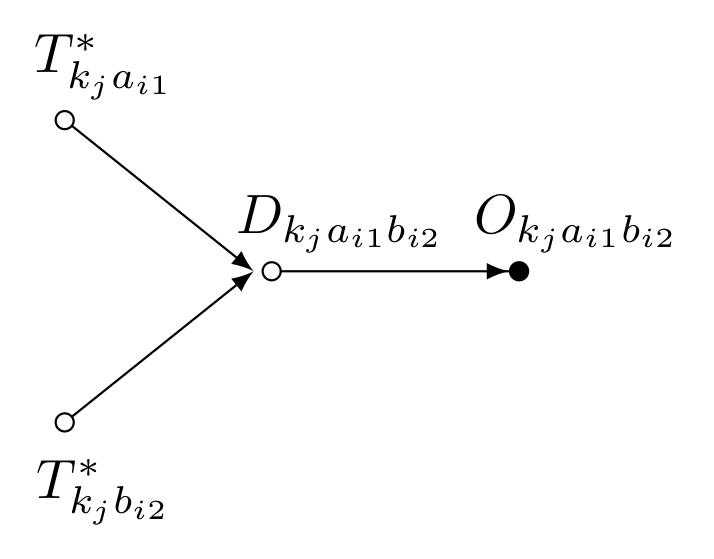
\includegraphics[width=0.3\linewidth,height=\textheight,keepaspectratio]{./images/png/CJ_TM_A2.png}

}

\caption{\label{fig-CJ_TM_A2}}

\end{figure}%

\paragraph{Figure 5}

\begin{figure}

\centering{

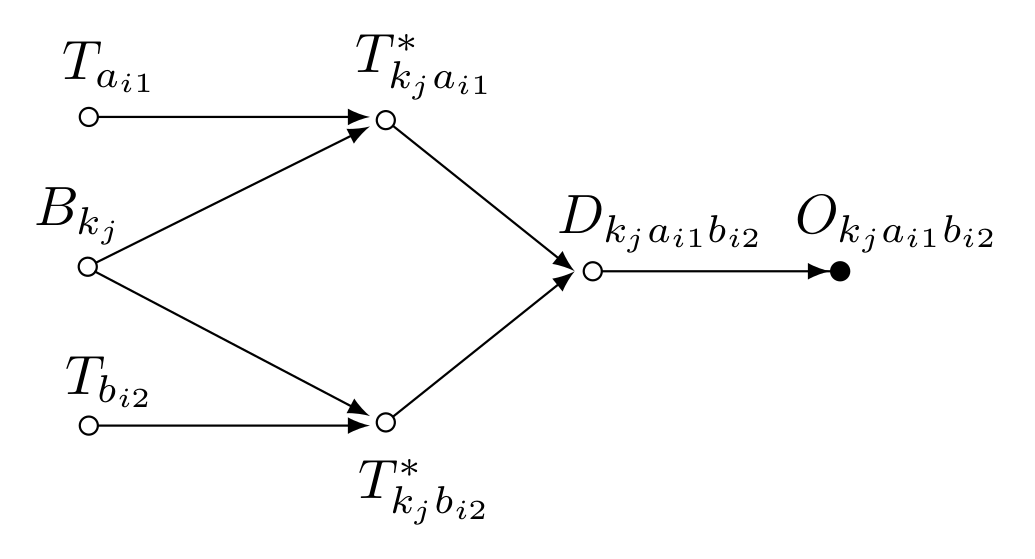
\includegraphics[width=0.42\linewidth,height=\textheight,keepaspectratio]{./images/png/CJ_TM_A3.png}

}

\caption{\label{fig-CJ_TM_A3}}

\end{figure}%

\paragraph{Figure 6}

\begin{figure}

\centering{

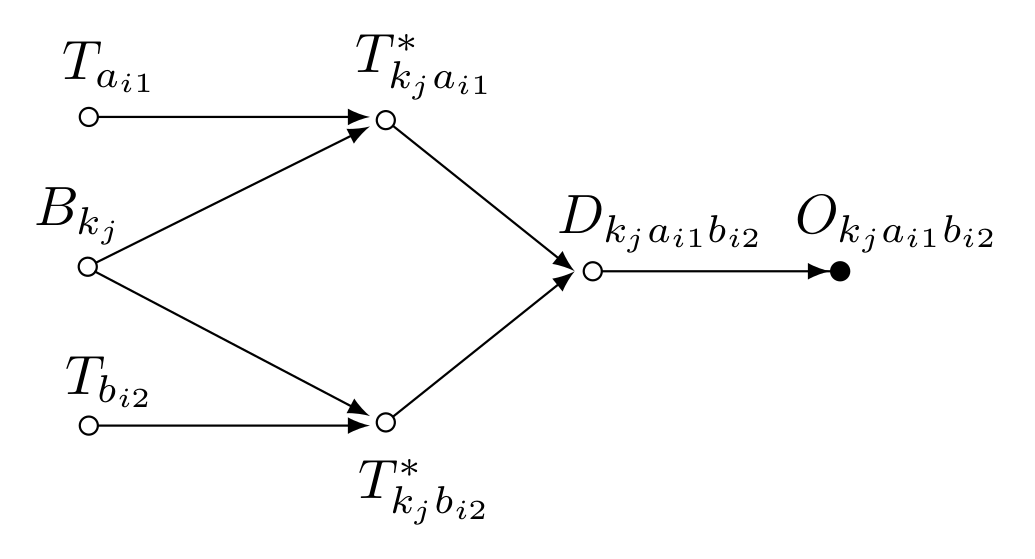
\includegraphics[width=0.42\linewidth,height=\textheight,keepaspectratio]{./images/png/CJ_TM_A4.png}

}

\caption{\label{fig-CJ_TM_A4}}

\end{figure}%

without loosing generality, the (latent) ``perceived'' and ``true''
discriminal processes for the stimuli can be depicted in a vector for
each judge, as in

\paragraph{Figure 7}

\begin{figure}

\centering{

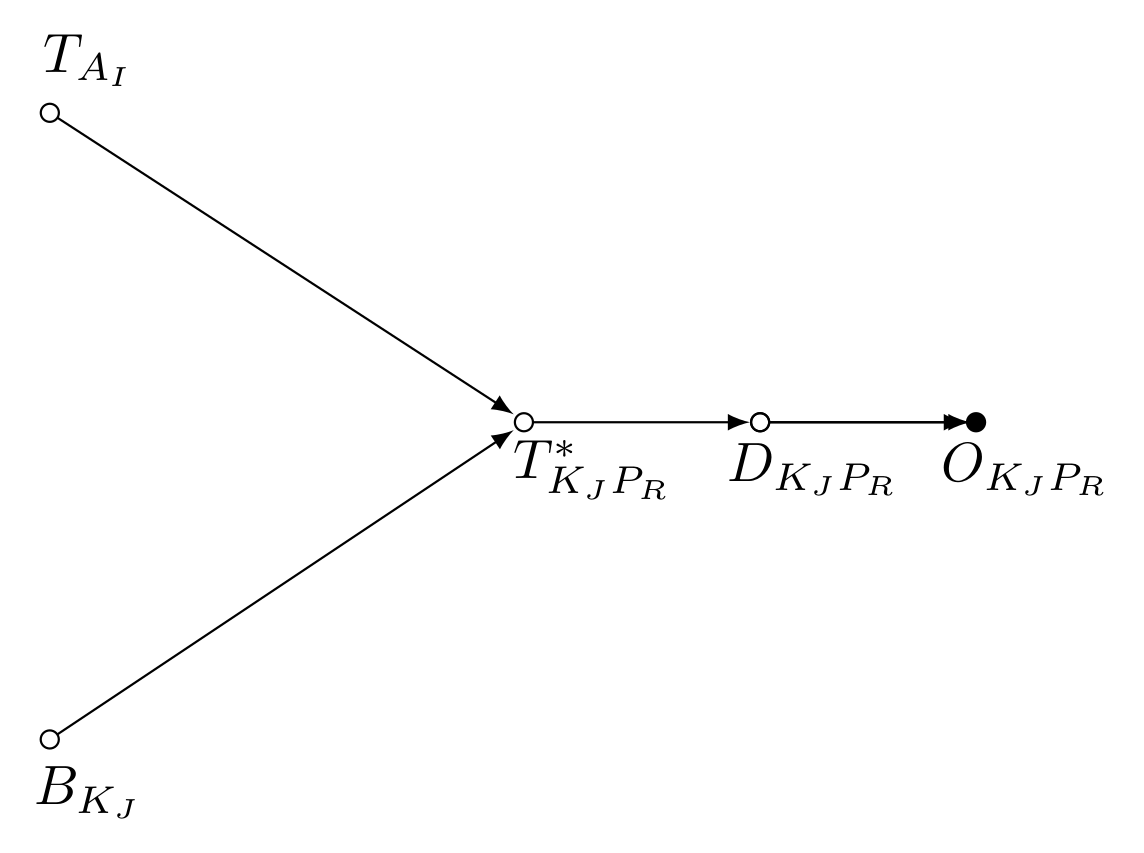
\includegraphics[width=0.42\linewidth,height=\textheight,keepaspectratio]{./images/png/CJ_TM_B1.png}

}

\caption{\label{fig-CJ_TM_B1}}

\end{figure}%

\paragraph{Figure 8}

\begin{figure}

\centering{

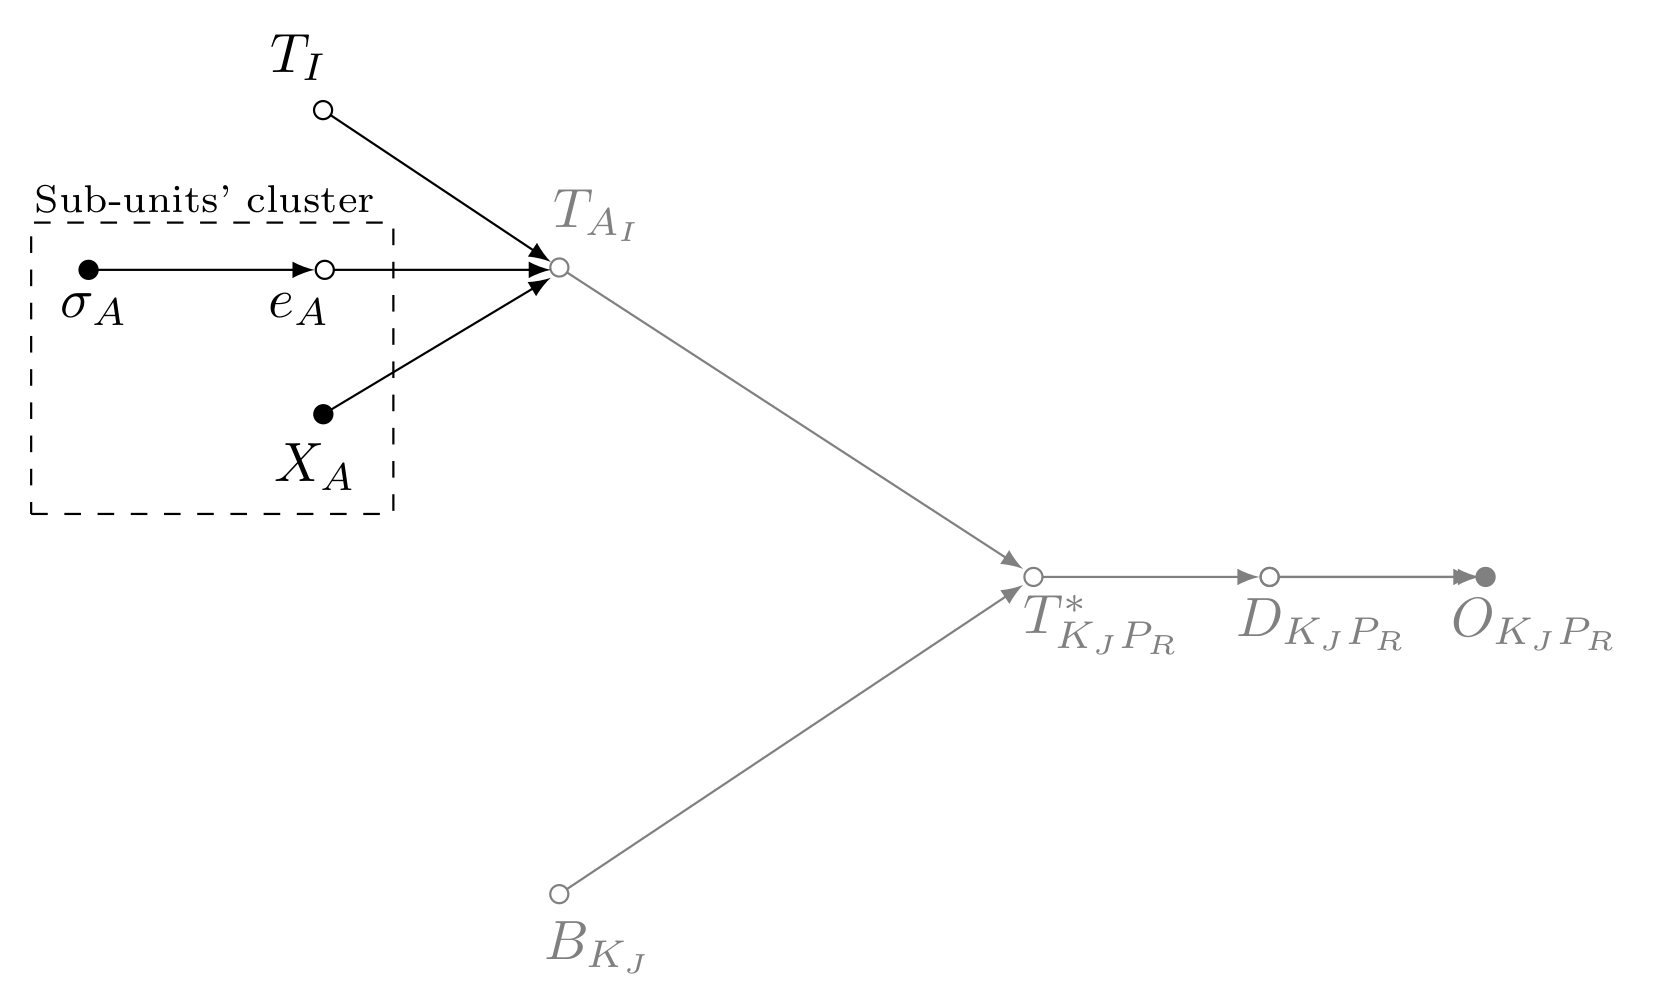
\includegraphics[width=0.62\linewidth,height=\textheight,keepaspectratio]{./images/png/CJ_TM_B2.png}

}

\caption{\label{fig-CJ_TM_B2}}

\end{figure}%

\paragraph{Figure 9}

\begin{figure}

\centering{

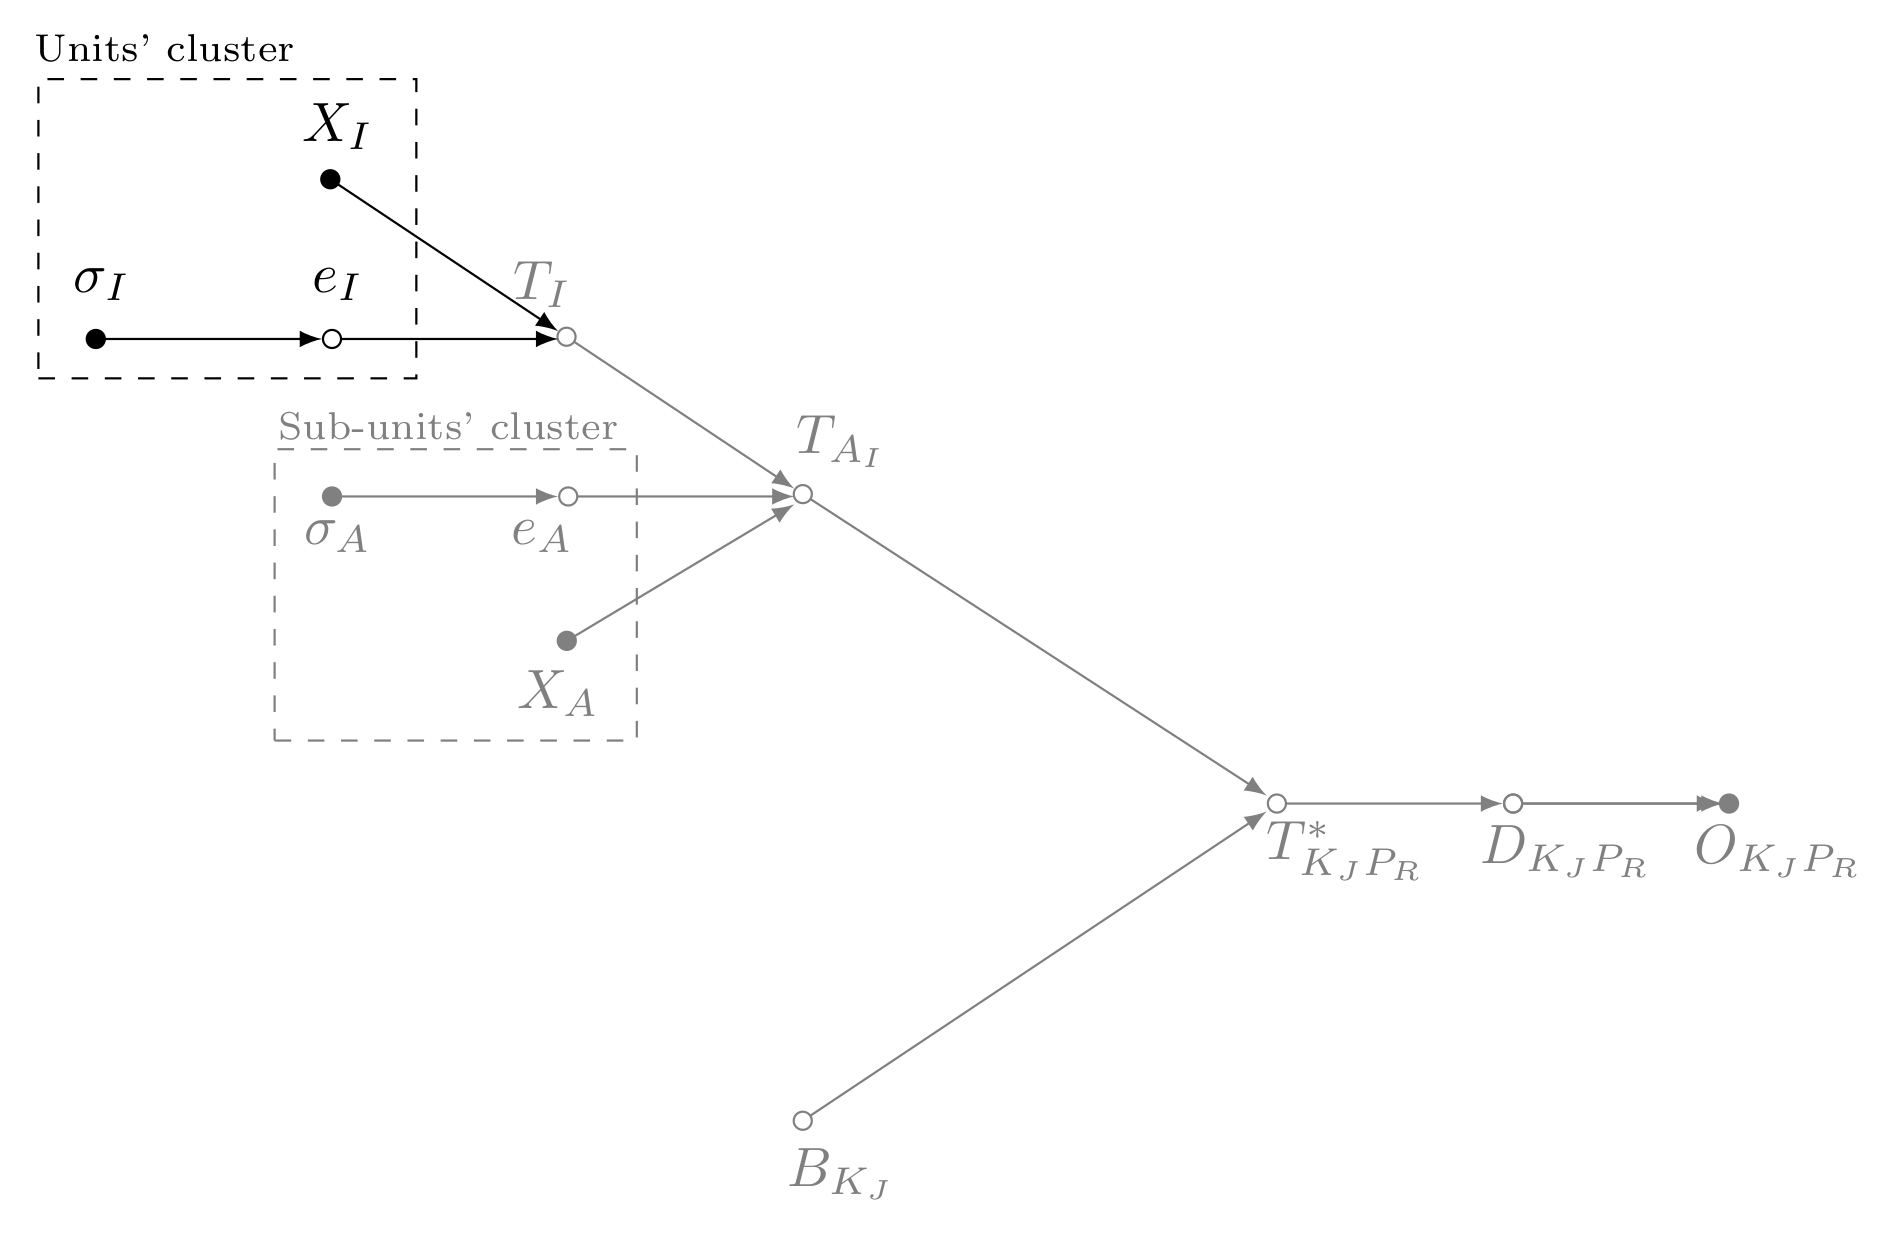
\includegraphics[width=0.72\linewidth,height=\textheight,keepaspectratio]{./images/png/CJ_TM_B3.png}

}

\caption{\label{fig-CJ_TM_B3}}

\end{figure}%

\paragraph{Figure 10}

\begin{figure}

\centering{

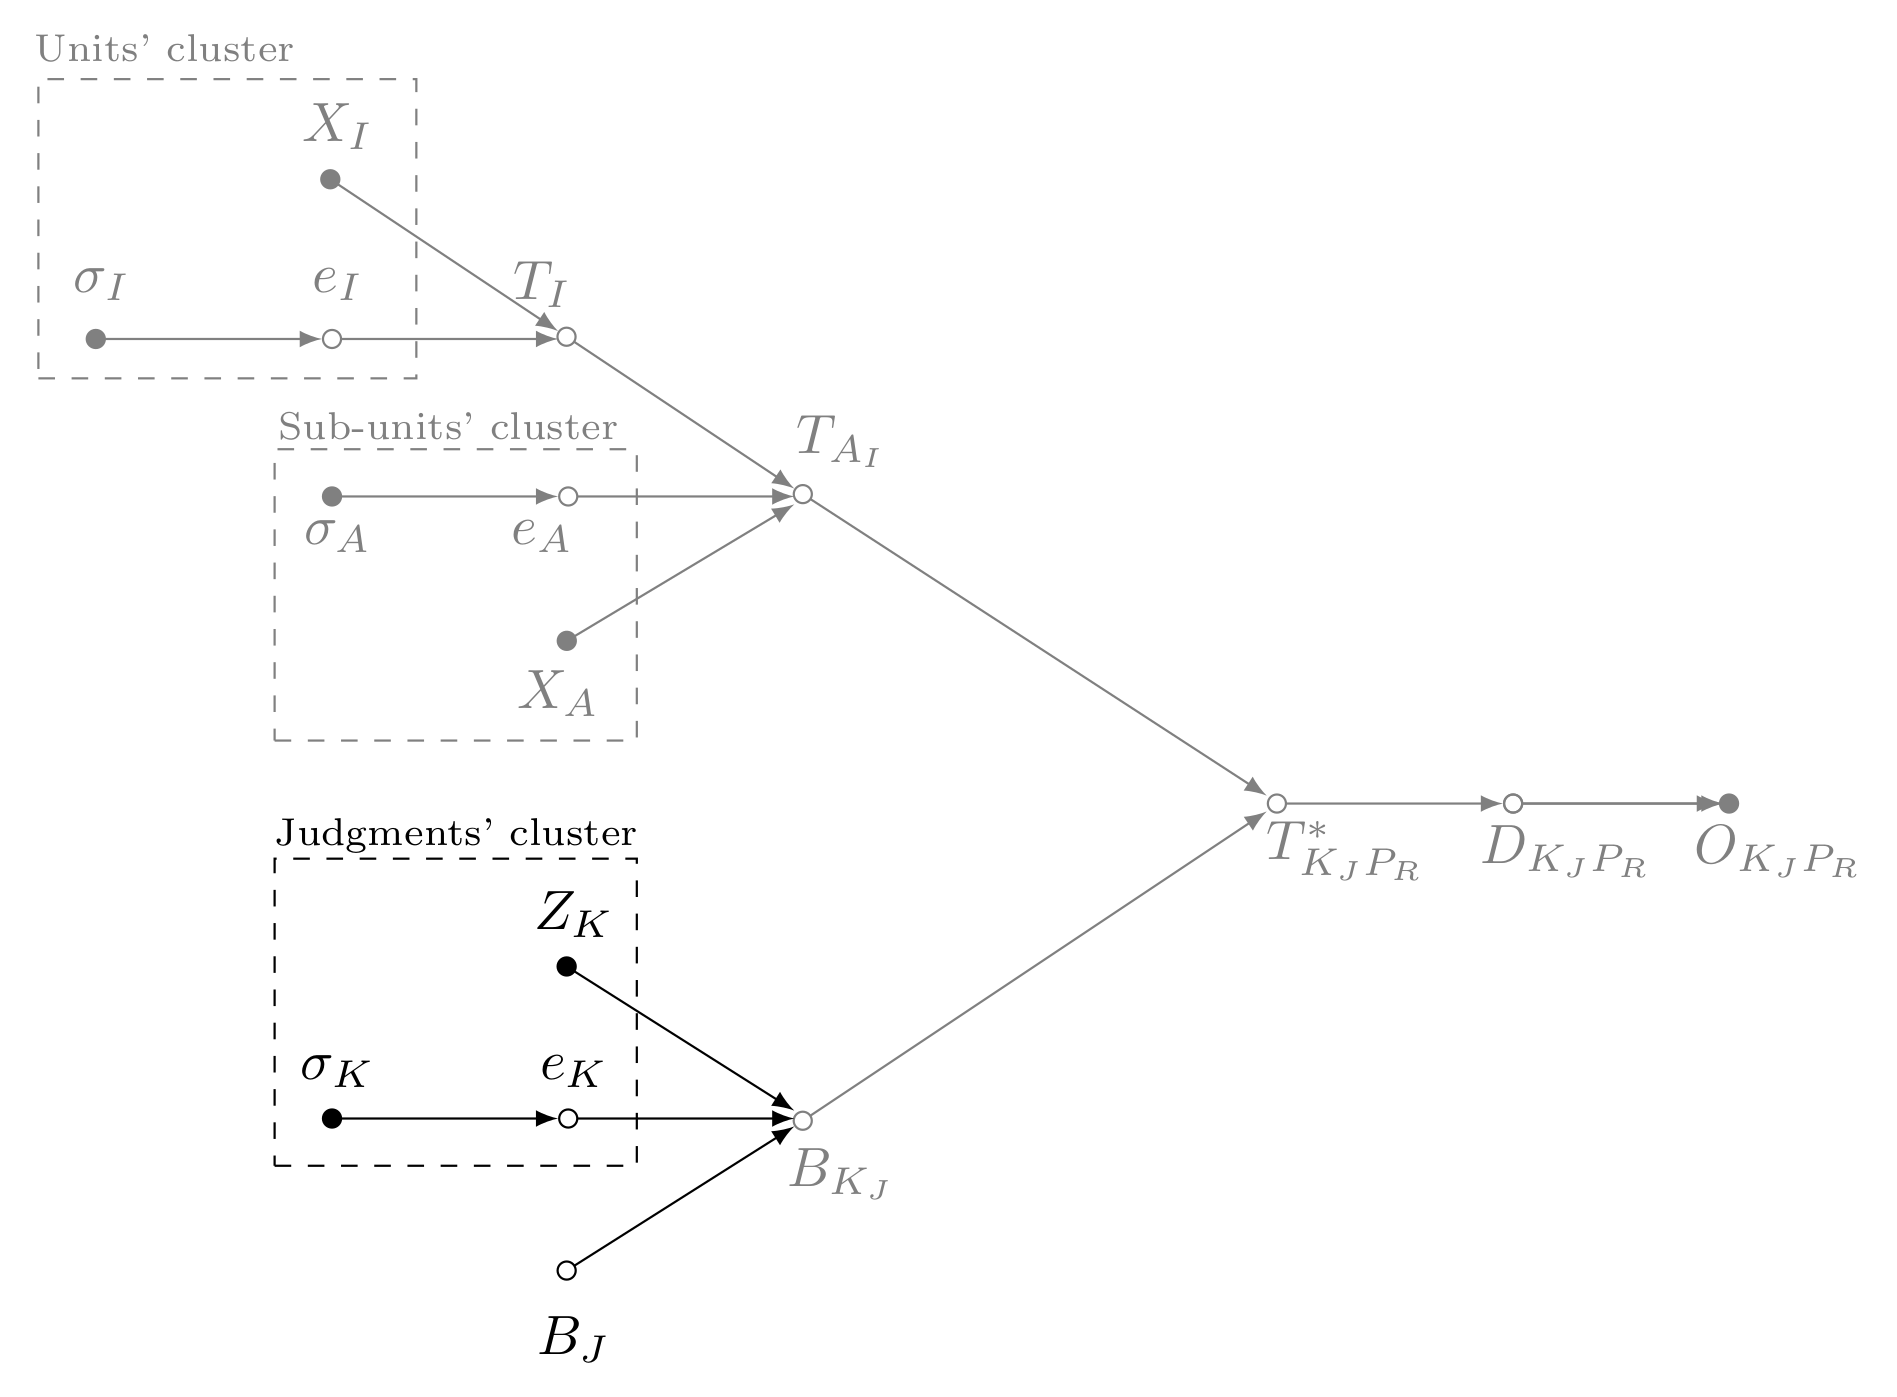
\includegraphics[width=0.72\linewidth,height=\textheight,keepaspectratio]{./images/png/CJ_TM_B4.png}

}

\caption{\label{fig-CJ_TM_B4}}

\end{figure}%

\paragraph{Figure 11}

\begin{figure}

\centering{

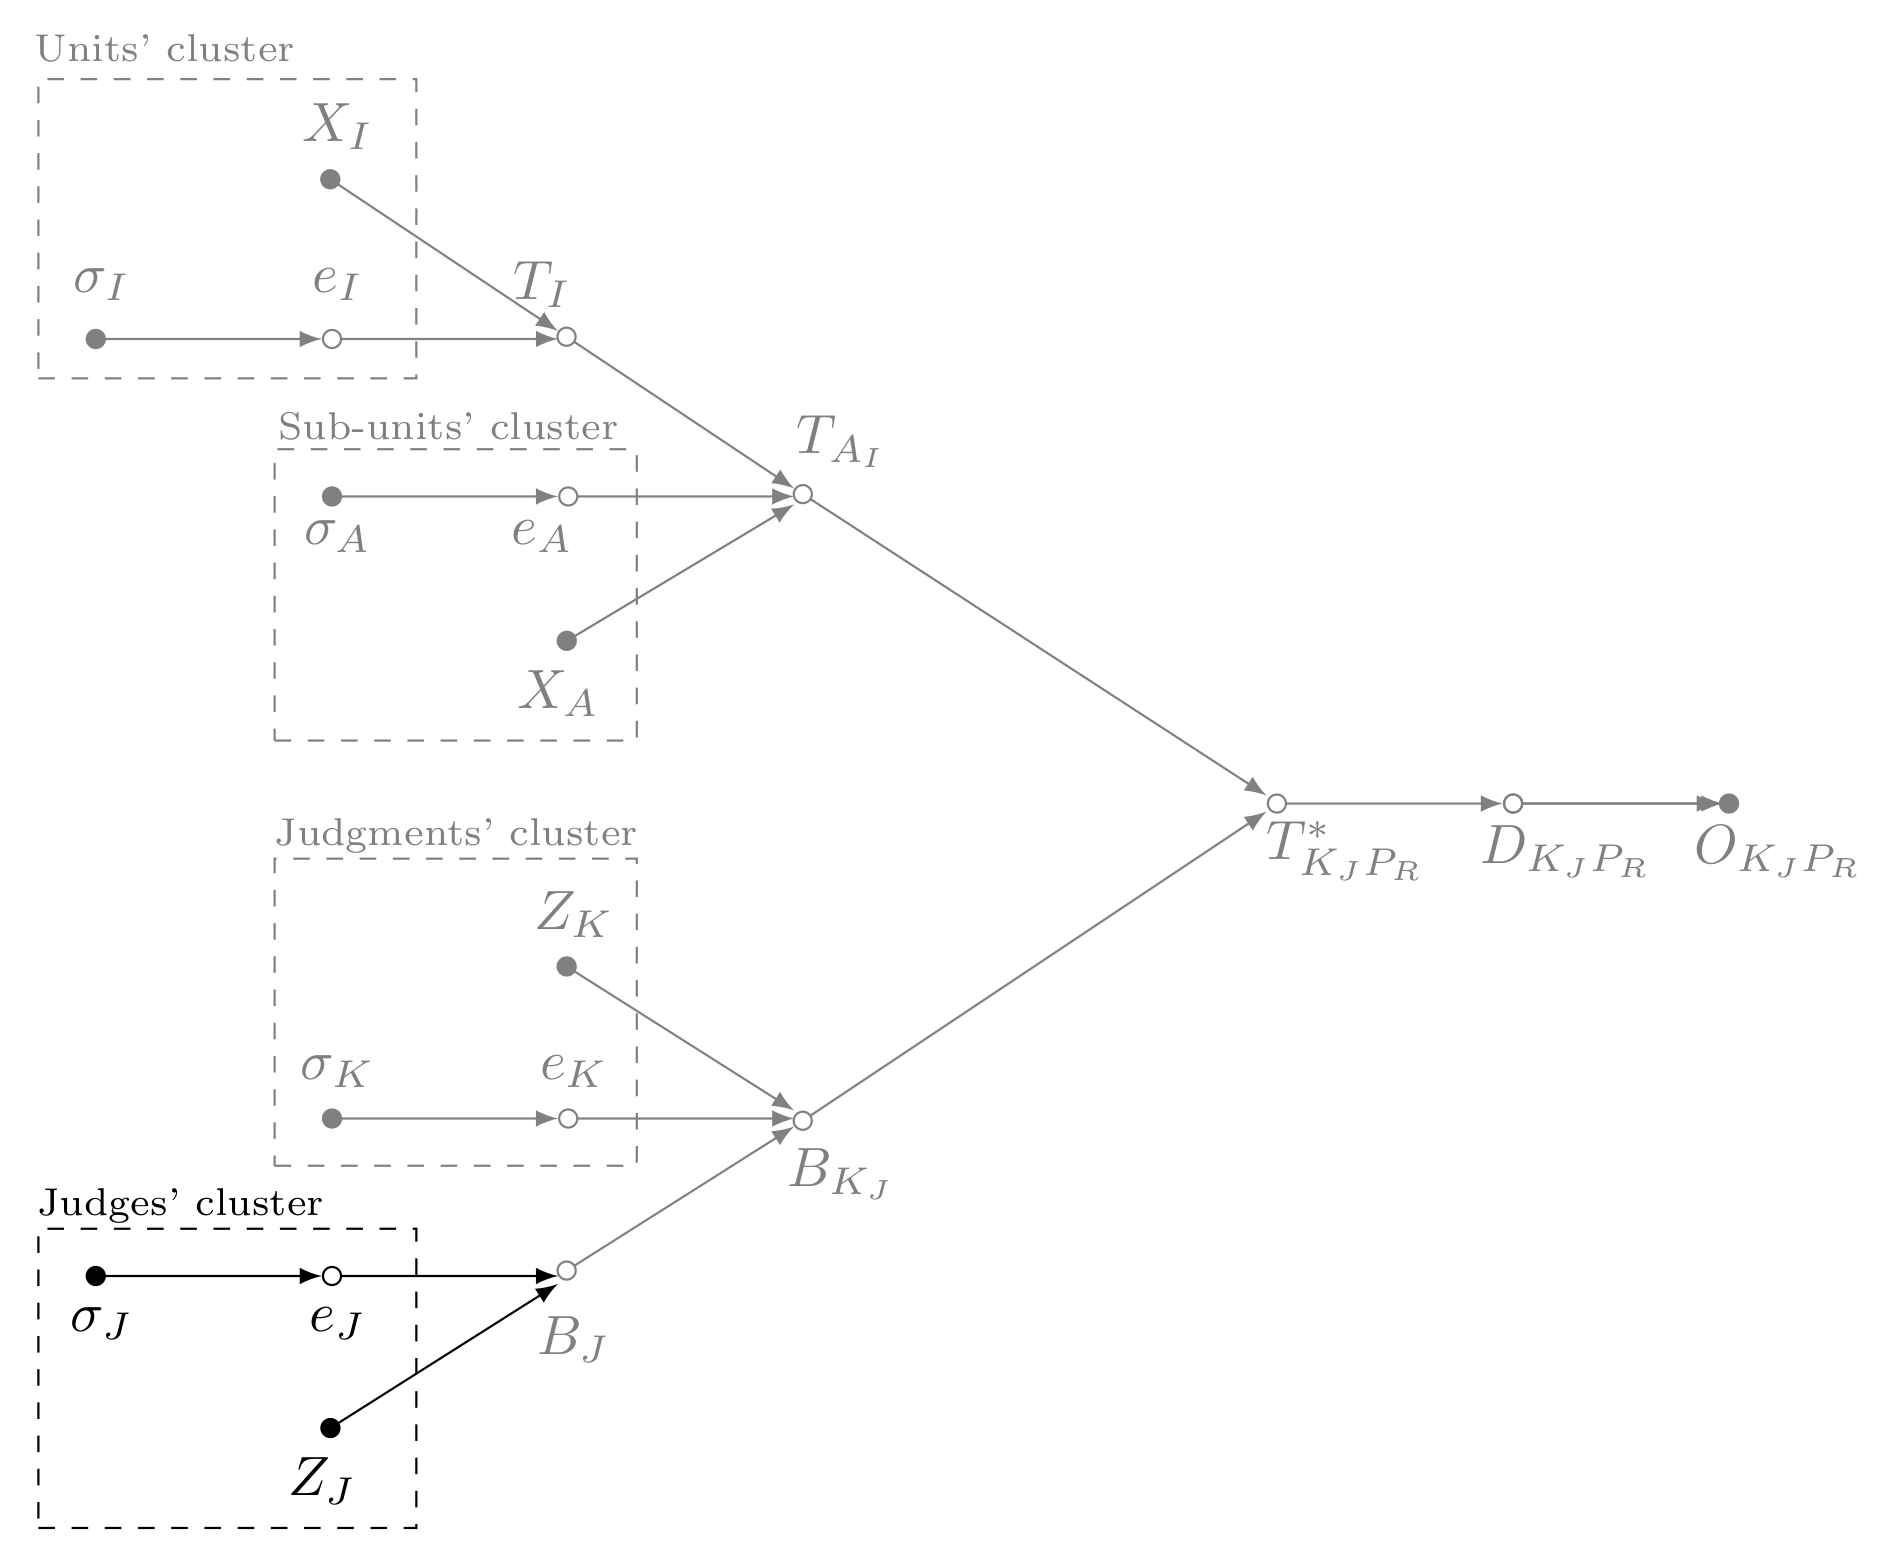
\includegraphics[width=0.72\linewidth,height=\textheight,keepaspectratio]{./images/png/CJ_TM_B5.png}

}

\caption{\label{fig-CJ_TM_B5}}

\end{figure}%

\paragraph{Figure 12}

\begin{figure}

\centering{

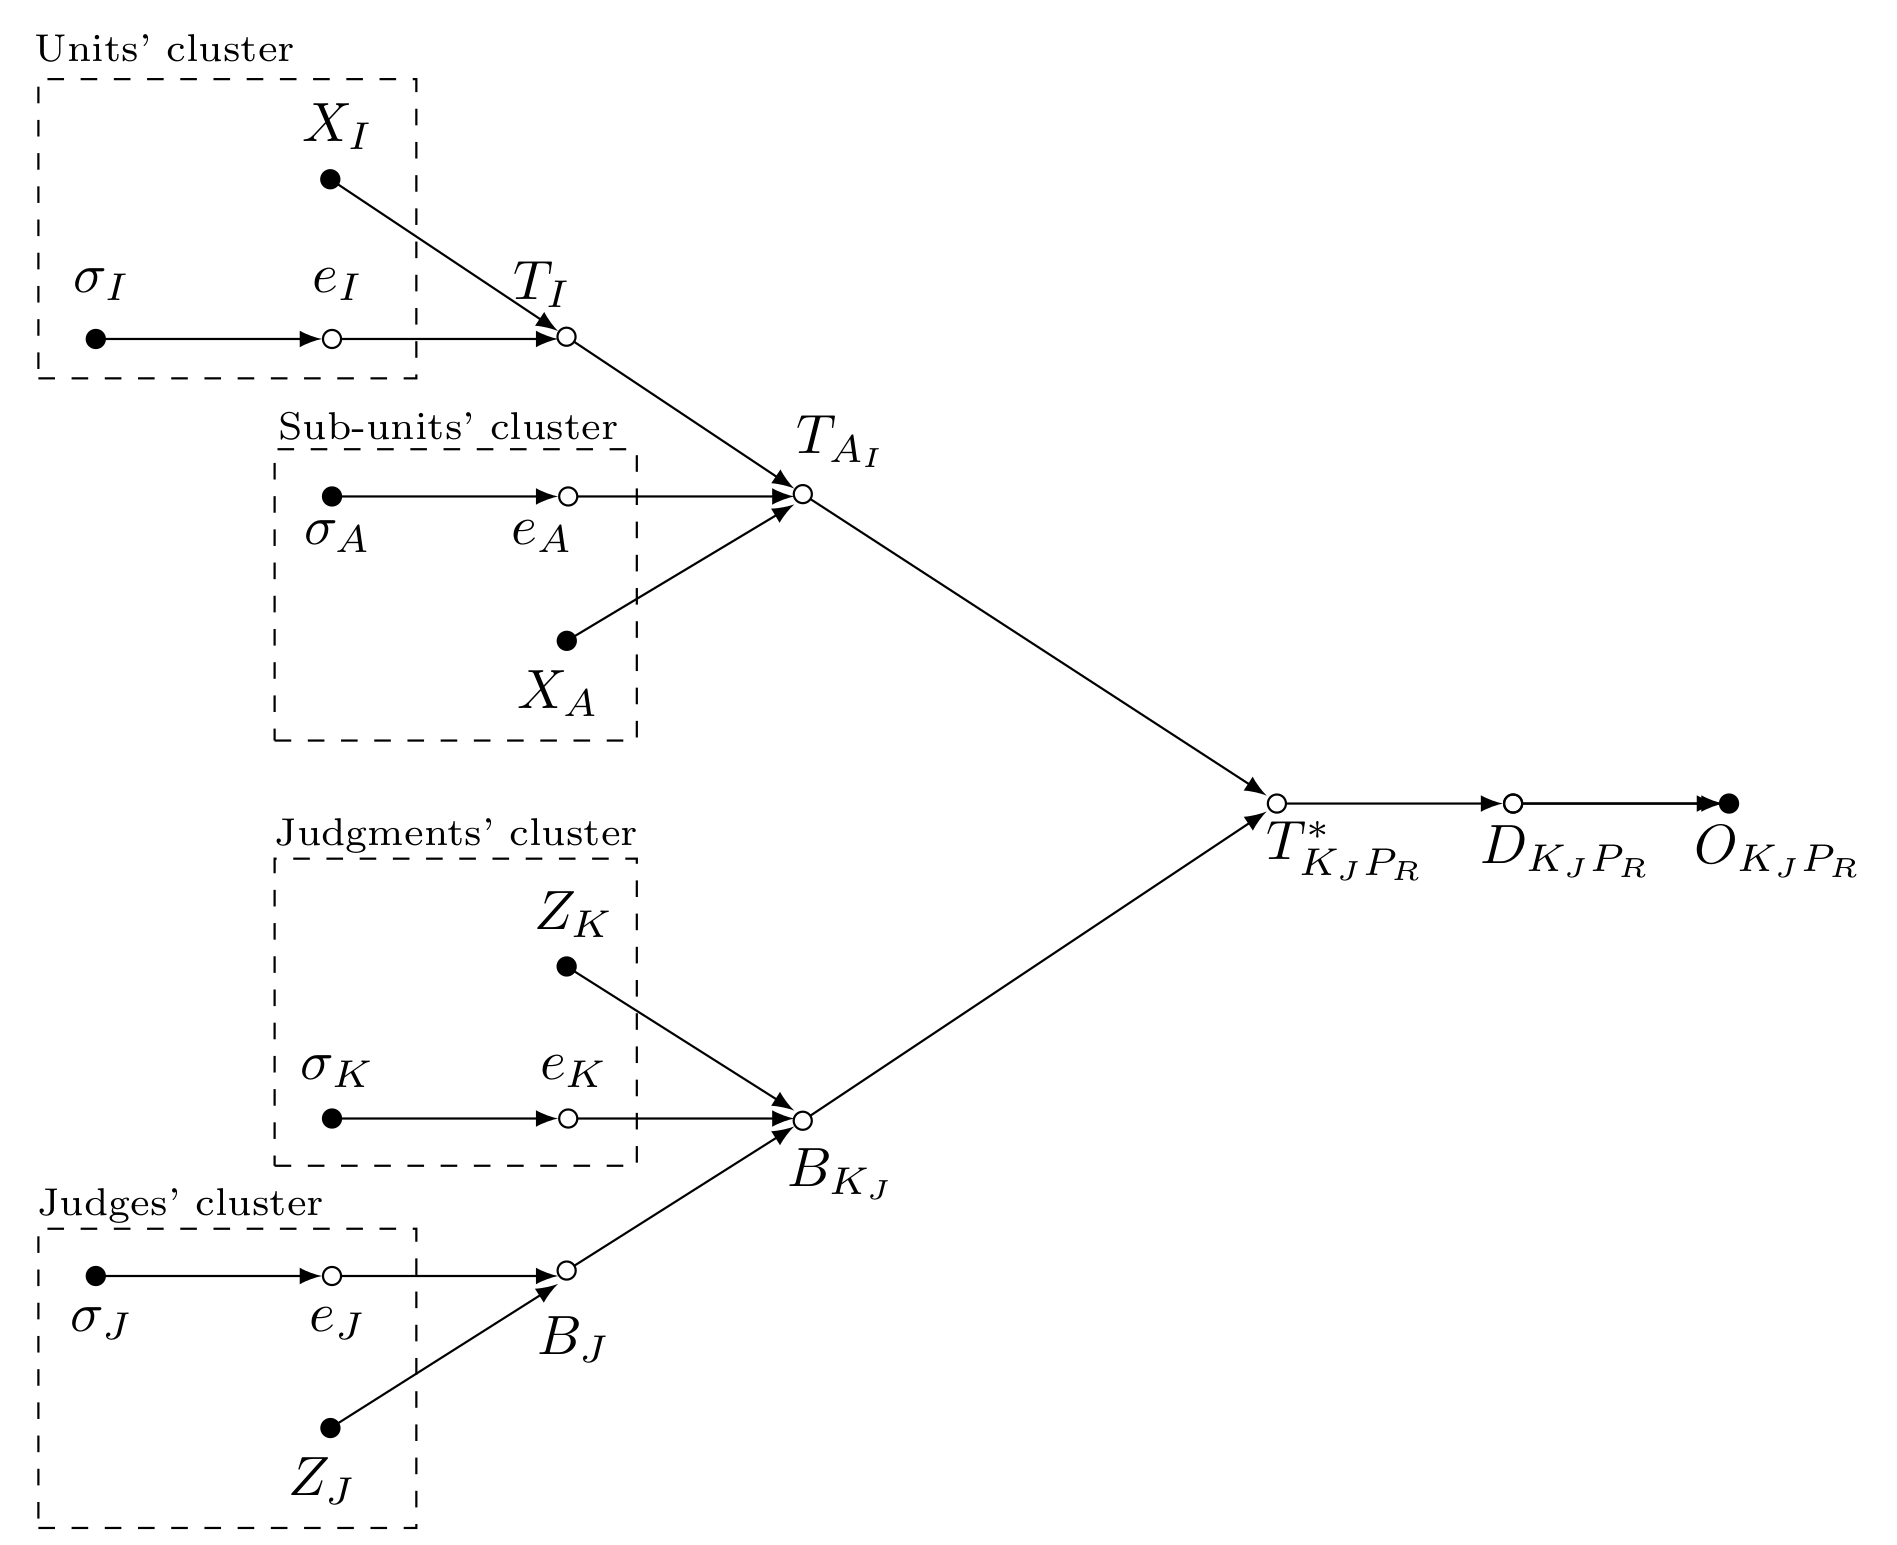
\includegraphics[width=0.72\linewidth,height=\textheight,keepaspectratio]{./images/png/CJ_TM_B6.png}

}

\caption{\label{fig-CJ_TM_B6}}

\end{figure}%

Considering the sampling process

\paragraph{Figure 13}

\begin{figure}

\centering{

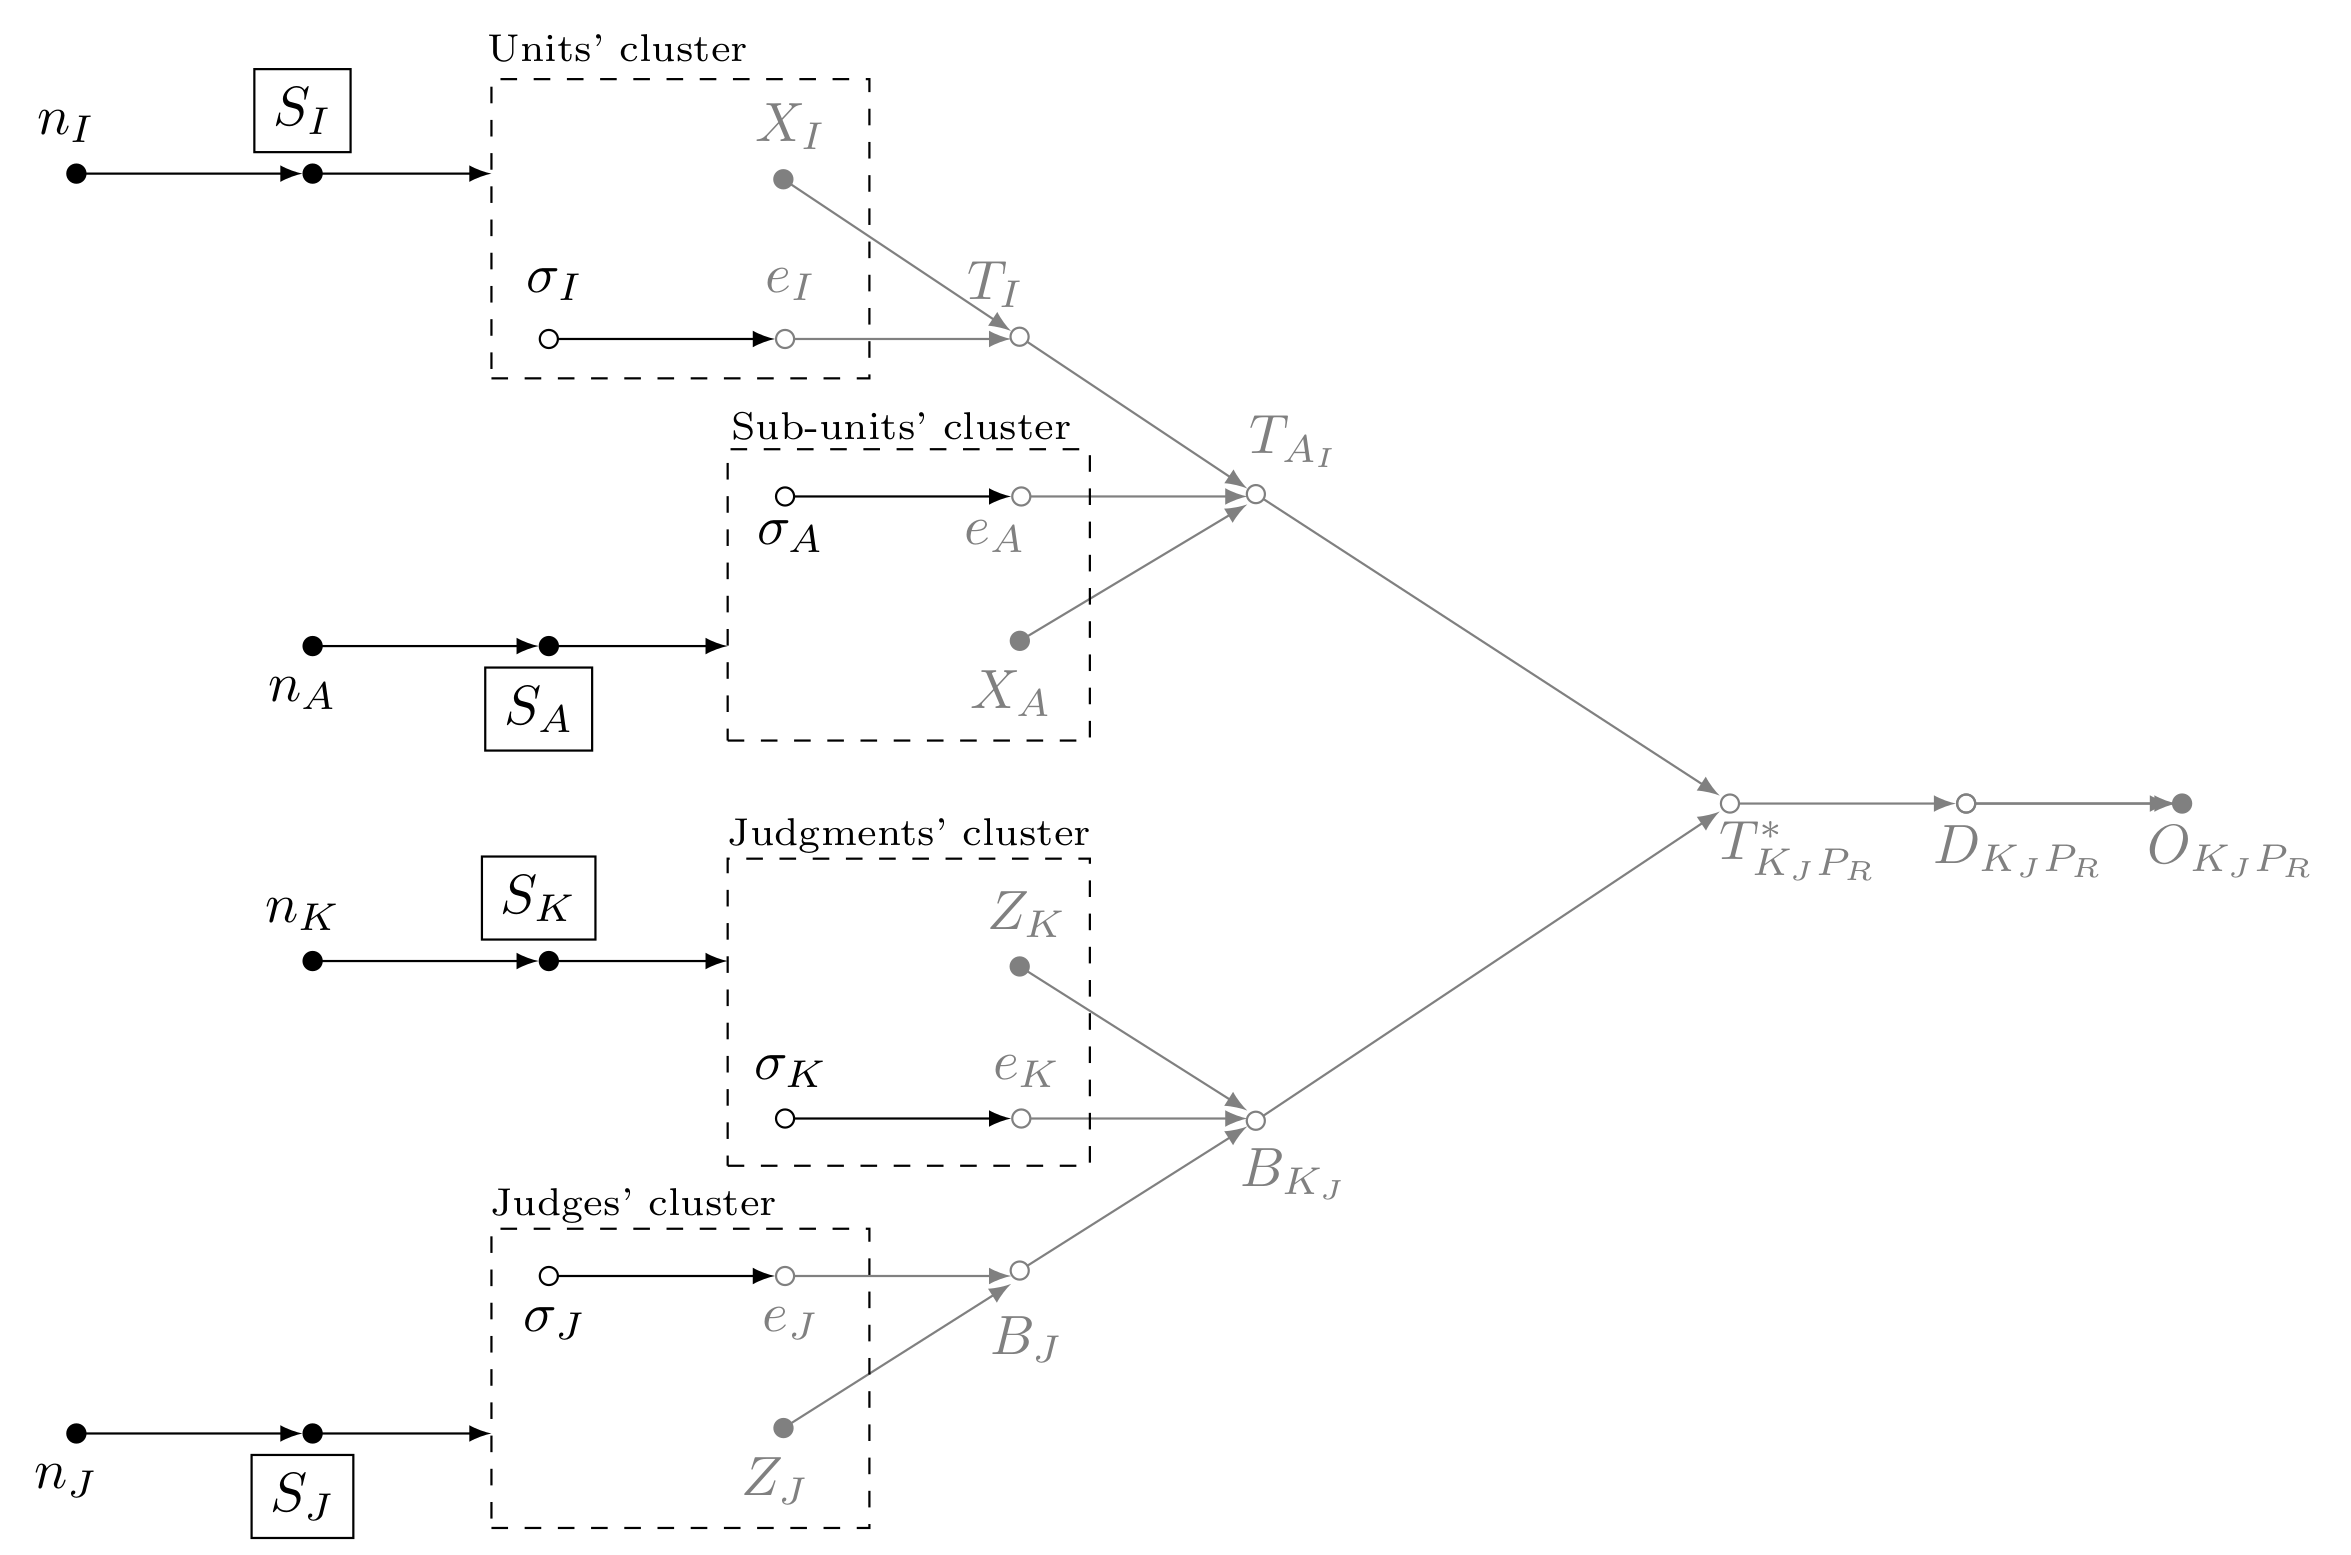
\includegraphics[width=0.9\linewidth,height=\textheight,keepaspectratio]{./images/png/CJ_TM_B7.png}

}

\caption{\label{fig-CJ_TM_B7}}

\end{figure}%

\paragraph{Figure 14}

\begin{figure}

\centering{

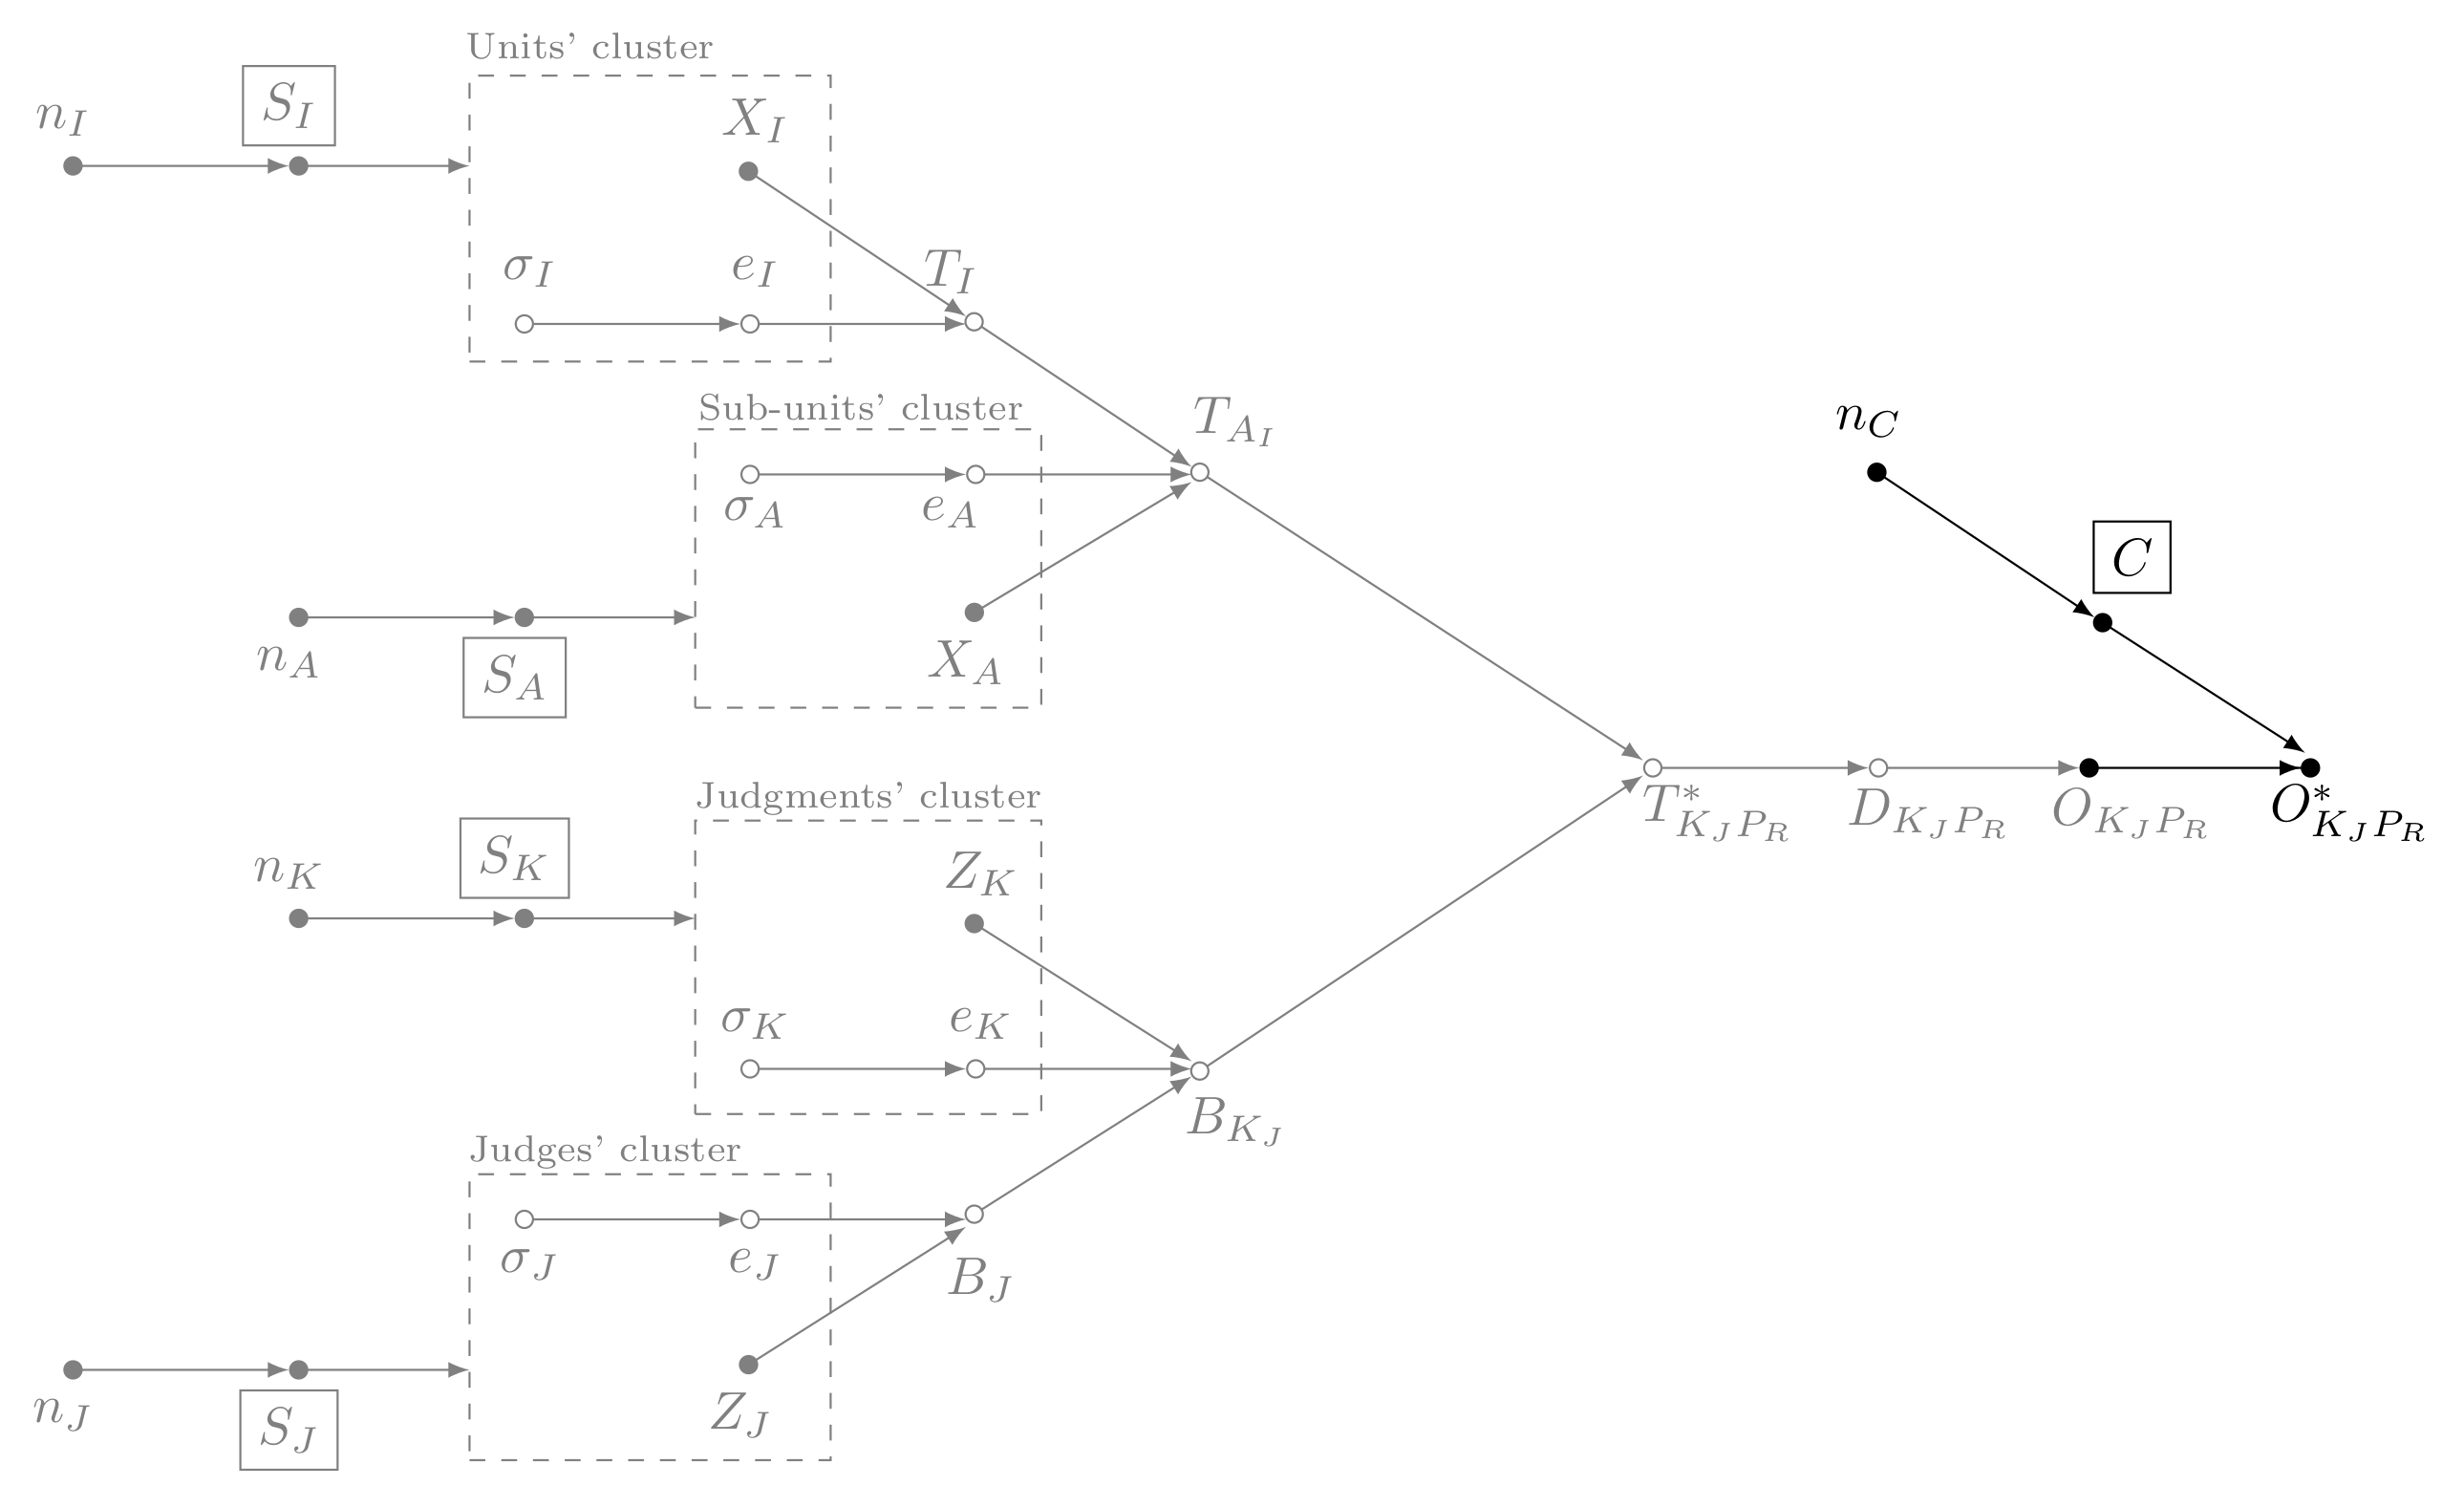
\includegraphics[width=1\linewidth,height=\textheight,keepaspectratio]{./images/png/CJ_TM_B8.png}

}

\caption{\label{fig-CJ_TM_B8}}

\end{figure}%

\paragraph{Figure 15}

\begin{figure}

\centering{

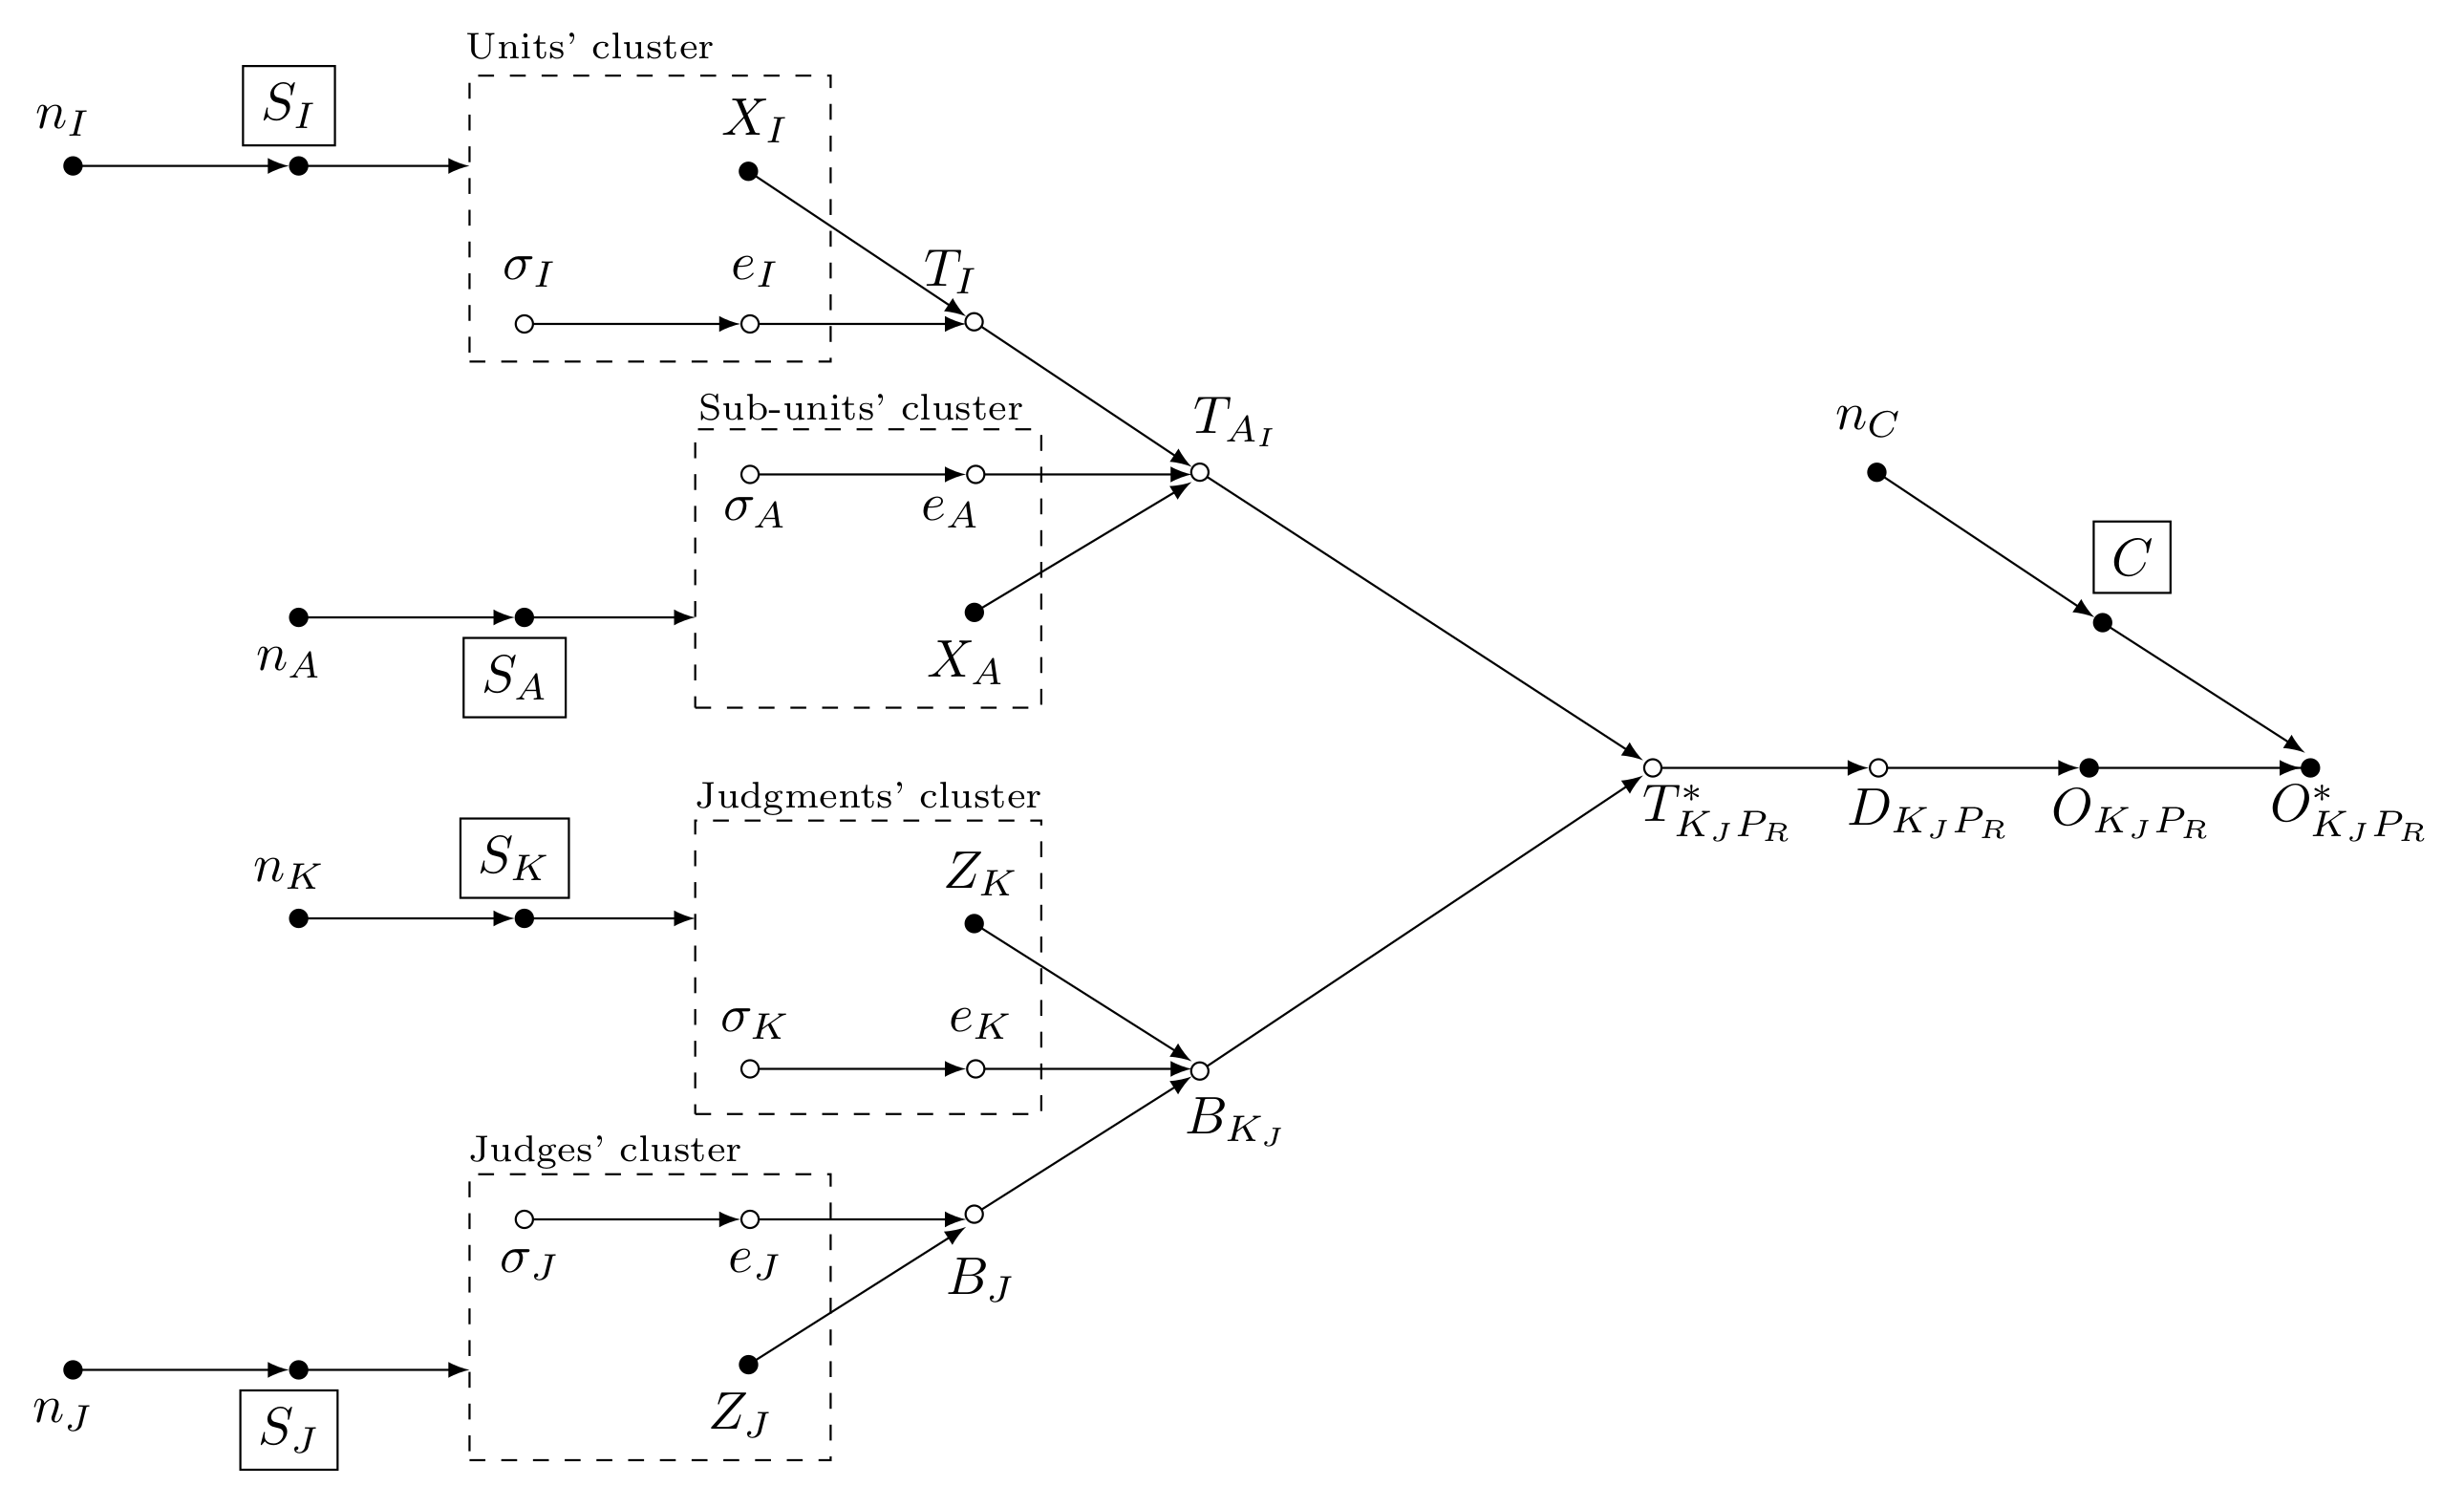
\includegraphics[width=1\linewidth,height=\textheight,keepaspectratio]{./images/png/CJ_TM_B9.png}

}

\caption{\label{fig-CJ_TM_B9}}

\end{figure}%

\subsection{From theory to statistics}\label{sec-theory-statistics}

\section{Discussion}\label{sec-discuss}

\subsection{Findings}\label{sec-discuss-finding}

\subsection{Limitations and further
research}\label{sec-discuss-limitations}

\section{Conclusion}\label{sec-conclusion}

\newpage{}

\section*{Declarations}\label{declarations}
\addcontentsline{toc}{section}{Declarations}

\textbf{Funding:} The project was founded through the Research Fund of
the University of Antwerp (BOF).

\textbf{Financial interests:} The authors have no relevant financial
interest to disclose.

\textbf{Non-financial interests:} The authors have no relevant
non-financial interest to disclose.

\textbf{Ethics approval:} The University of Antwerp Research Ethics
Committee has confirmed that no ethical approval is required.

\textbf{Consent to participate:} Not applicable

\textbf{Consent for publication:} All authors have read and agreed to
the published version of the manuscript.

\textbf{Availability of data and materials:} No data was utilized in
this study.

\textbf{Code availability:} All the code utilized in this research is
available in the digital document located at:
\url{https://jriveraespejo.github.io/paper2_manuscript/}.

\textbf{AI-assisted technologies in the writing process:} The authors
utilized a range of AI-based language tools throughout the preparation
of this work. They occasionally employed the tools to refine phrasing
and optimize wording, ensuring appropriate language use and enhancing
the manuscript's clarity and coherence. The authors take full
responsibility for the final content of the publication.

\textbf{CRediT authorship contribution statement:}
\emph{Conceptualization:} S.G., S.DM., T.vD., and J.M.R.E;
\emph{Methodology:} S.DM., T.vD., and J.M.R.E; \emph{Software:}
J.M.R.E.; \emph{Validation:} J.M.R.E.; \emph{Formal Analysis:} J.M.R.E.;
\emph{Investigation:} J.M.R.E; \emph{Resources:} S.G., S.DM., and T.vD.;
\emph{Data curation:} J.M.R.E.; \emph{Writing - original draft:}
J.M.R.E.; \emph{Writing - review and editing:} S.G., S.DM., and T.vD.;
\emph{Visualization:} J.M.R.E.; \emph{Supervision:} S.G. and S.DM.;
\emph{Project administration:} S.G. and S.DM.; \emph{Funding
acquisition:} S.G. and S.DM.

\newpage{}

\section*{References}\label{references}
\addcontentsline{toc}{section}{References}

\renewcommand{\bibsection}{}
\bibliography{references.bib}





\end{document}
